\chapter{Динамическое программирование}

\begin{note}
	\definitionfont{Динамическое программирование} --- метод решения сложных задач путём разбиения их на более простые подзадачи. Этот метод эффективен, если процесс принятия  решения состоит из многих шагов, то есть когда итоговое решение --- последовательность принимаемых решений (\definitionfont{стратегия}). Теоретически с помощью динамического программирования можно решить любую экстремальную задачу, однако практически это не всегда возможно, так как появляется слишком много состояний.
\end{note}

\section{Задача загрузки судна}

Начнём рассмотрение динамического программирования на примере задачи.

\problem[загрузки судна]\label{pr:loading_vessel}

Пусть есть грузовое судно и набор различных контейнеров. Требуется загрузить судно контейнерами таким образом, чтобы при их дальнейшей продаже заработать как можно больше, при этом размер грузовой площадки судна ограничен.

\mathmodel

\textbf{1. Что будем оптимизировать?} Ответ: доход с продажи контейнеров должен быть максимальным.

\bigskip

\textbf{2. Что существенно влияет на оптимизируемую характеристику?}

Пусть $i=1 \dots N$ --- номера контейнеров.

\bigskip

\textit{Параметры}

\begin{itemize}[nosep]
	\item $h_i$ --- место на грузовой площадке, занимаемое контейнером $i$;
	
	\item $c_i$ --- ценность контейнера $i$;
	
	\item $P$ --- размер грузовой площадки судна.
\end{itemize}

\bigskip

\textit{Переменные}
\begin{itemize}[nosep]
	\item $x_i$ --- сколько контейнеров с номером $i$ нужно взять на судно.
\end{itemize}

\begin{figure}[H]
	\centering
	\def\svgwidth{\linewidth}
	\fbox{\input{./graphics/cargo_ship_1_N.pdf_tex}}
\end{figure}

\bigskip

\textbf{3. Математическая формулировка задачи}

\[
\sum_{i=1}^{N} c_i x_i \to \max_{(x_i), \; i \in \{1, \dots, N\}},
\]
\[
\sum_{i=1}^{N} h_i x_i \le P,
\]
\[
x_i \in \{0, 1, 2, 3, \dots\}, \quad i \in {1, \dots N}.
\]

\solution

Для решения задачи будем рассматривать семейства аналогичных задач. Каждое семейство будет охарактеризовываться парой $(n, p)$, где $p$ --- место на площадке, а $n$ --- минимальный номер для контейнеров, которые у нас есть. То есть вместо рассмотрения исходной задачи про все $N$ контейнеров и всю грузовую площадку размером $P$ будем рассматривать задачи, в которых нам доступны не все контейнеры, а лишь начинающиеся с номера $n \le N$, а также в которых нам доступна не вся грузовая площадка судна, а лишь её часть размером $p \le P$.

\begin{figure}[H]
	\centering
	\def\svgwidth{\linewidth}
	\fbox{\input{./graphics/cargo_ship_n_N.pdf_tex}}
\end{figure}

Запишем \underline{целевую функцию} и \underline{ограничения} для семейства $(n, p)$
\[
\sum_{i=n}^{N} c_i x_i \to \max_{(x_i), \; i=n \dots N},
\]
\[
\sum_{i=n}^{N} h_i x_i \le p,
\]
\[
x_i \in \{0, 1, 2, 3, \dots\} \quad i = n \dots N.
\]

Зададимся вопросом: а есть ли в этом семействе задачи, которые можно легко решить? Да, например если $n = N$, то есть если у нас в распоряжении есть лишь контейнер с номером $N$.

Введём обозначение. Пусть $f_n(p)$ --- оптимальное значение целевой функции семейства задач $(n, p)$. По своей сути $f_n(p)$ --- это максимальный доход, который мы получим, если будем на площадку размера $p$ грузить контейнеры с номерами $n, n+1, n+2, \dots, N$. Легко заметить, что
\[
f_N(p) = c_N \cdot \bigg[\frac{p}{h_N}\bigg].
\]

Действительно, если у нас в распоряжении есть лишь контейнеры с номером $N$, то для получения максимального дохода нужно попытаться по-максимуму загрузить ими площадку на грузовом корабле, $\big[\frac{p}{h_N}\big]$ --- количество контейнеров, которое поместится на площадку.

Таким образом, мы уже умеем решать задачу $(N, p)$ для любого $p \le P$. Теперь нужно совершить переход к решению исходной задачи
\[
f_N(p) \longrightarrow f_1(P).
\]

Для этого сформулируем принцип.

\definition[принцип оптимальности для оптимальной стратегии]

\definitionfont{Оптимальная стратегия обладает тем свойством, что каким бы не было первое решение, последующие решения должны образовывать оптимальную стратегию относительно состояния, полученного по итогам первого решения}.

\example

Пусть мы стоим у доски и нам захотелось как можно быстрее выйти из аудитории через дверь. Каким бы ни был наш первый шаг, если мы хотим дойти до двери как можно быстрее, придётся всё время действовать оптимально. То есть даже если первый шаг был оптимальным, но потом мы пошли неоптимально, стратегия точно не получится оптимальной.

\returntoproblem

Предположим, что для некоторого $n \le N$ и для $p \le P$ мы уже знаем
\[
f_{n+1}(p), f_{n+2}(p), \dots, f_{N}(p),
\]

однако нам бы хотелось посчитать $f_n(p)$, как это можно сделать?

Предположим, что $x_n = x = 1$, тогда груз с номером $n$ даст нам ценность $c_n \cdot x = c_n$ и займёт на площадке место $h_n \cdot x = h_n$. Обобщим для $x_n \neq 1$ и запишем целевую функцию
\[
\boxed{\forall p \le P \quad f_n(p) = \max_{h_n \cdot x \le p, \; x = 0, 1, 2, \dots} \big\{c_n \cdot x + f_{n+1}(p - h_n \cdot x)\big\}}.
\]

Действительно, оптимальное значение при имеющихся контейнерах $n, n+1, n+2, \dots, N$ складывается из некоторого количества контейнеров с номером $n$ и контейнеров $n+1, n+2, \dots, N$. Чтобы найти оптимальное значение нужно перебрать все варианты того, сколько взять контейнеров с номером $n$, при этом ясно, что взять их <<слишком много>> не получится, потому что размер площадки ограничен $p$. Это условие отражается через $h_n \cdot x \le p$.

Мы получили \textbf{рекуррентное соотношение динамического программирования}, при этом, как уже говорилось ранее, $f_n(p)$ можно получить перебором значение $x_n = x$, а $f_{n+1}(\dots)$ по предположению нам уже известно.

Таким образом, для решения исходной задачи нужно для всех $p \le P$ и для всех $n = 2 \dots N$ найти значение $f_n(p)$, а затем вычислить $f_1(P)$, это и будет значение целевой функции исходной задачи. Для получения стратегии нужно использовать значения $\{x_n\}_{i=1}^N$, на которых на каждом шаге достигается максимум $f_n(p)$.

\begin{note}
	Почему мы предполагаем, что $f_{n+1}(\dots)$ нам известно? Ранее мы обсуждали, что мы можем вычислить $f_N(p)$ для любого $p \le P$. Значит с помощью рекуррентного соотношения можем вычислить $f_{N-1}(p)$ для любого $p$, после этого можно вычислить $f_{N-2}(p)$ и так далее. То есть, если у нас есть хотя бы одно значение <<в конце>>, то мы можем дойти до <<начала>> за определённое число шагов. Поэтому предположению о том, что на некотором шаге $n$ нам уже известно оптимальное значение $f_{n+1}(p)$ имеет место.
\end{note}

\section{$N$-шаговый процесс принятия решений}

Обобщим подход к решению \hyperref[pr:loading_vessel]{задачи о загрузке судна}.

\algorithm[$N$-шаговый процесс принятия решений]\label{alg:n_step_process}

\textbf{Исходные данные}

Для осуществления $N$-шагового процесса необходимо следующее

\begin{itemize}[nosep]
	\item \definitionfont{Количество шагов процесса}. Обозначение: $\boxed{N}$.
	
	\item \definitionfont{Состояние} --- некоторое значение, которое мы имеем в начале каждого шага. Обозначение: $\boxed{p}$.
	
	\item \definitionfont{Решение} на шаге $i$. Обозначение: $\boxed{q_i}$ ($i = 1 \dots N$).
	
	\item \definitionfont{Начальное состояние} --- некоторая известная заданная величина. Обозначение: $\boxed{p_0}$.
	
	\item \definitionfont{Множество возможных состояний} на шаге $i$. Обозначение: $\boxed{P_i}$ ($i = 1 \dots N+1$).
	
	\item \definitionfont{Множество возможных решений} на шаге $i$. Обозначение $\boxed{Q_i}$ ($i = 1 \dots N$).
	
	\item \definitionfont{Функция перехода} --- функция перехода из текущего состояния $p$ в новое состояние $p'$, если на $i$-ом шаге принимается решение $q$
	\[
	p' = \boxed{T_i(p, q)}.
	\]
	
	\item \definitionfont{Множество допустимых решений} на $i$-ом шаге в состоянии $p$
	\[
	\boxed{Q_i(p) = \{q \in Q_i \; \big| \; T_i(p, q) \in P_{i+1}\}}.
	\]
	
	\item $\boxed{f_n(p)}$ --- оптимальное значение целевой функции на шаге $n$, если в начале шага было состояние $p$.
\end{itemize}

\begin{note}
	В \hyperref[pr:loading_vessel]{задаче о загрузке судна}
	
	\begin{itemize}[nosep]
		\item \definitionfont{количество шагов процесса}: количество видов контейнеров;
		
		\item \definitionfont{состояние}: свободное место на грузовой площадке;
		
		\item \definitionfont{решение} на шаге $i$: сколько грузить контейнеров с номером $i$;
		
		\item \definitionfont{начальное состояние}: $P$ (свободное место на пустой грузовой площадке);
		
		\item \definitionfont{множество возможных состояний}: $\{0, 1, 2, \dots, P\}$ (сколько может быть доступного места на грузовой площадке на каждом шаге);
		
		\item \definitionfont{множество возможных решений}: $\{0, 1, 2, 3, \dots\}$ (это означает, что можно грузить лишь целое неотрицательное количество контейнеров);
		
		\item \definitionfont{функция перехода} на шаге $n$ в состоянии $p$, если принимается решение $q$: $(p - h_n \cdot q)$ (это означает, сколько свободного места останется на площадке, если сейчас свободно $p$ и грузим $q$ контейнеров типа $n$);
		
		\item \definitionfont{множество допустимых решений} на шаге $n$ в состоянии $p$: 
		\[
		Q_n(p) = \big\{q \in \{0, 1, 2, 3, \dots\} \; \big| \; h_n \cdot x \le p\big\}.
		\]
	\end{itemize}
\end{note}

\begin{note}
	Множества возможных состояний $P_i$ определены для $i = 1 \dots N+1$, хотя шага с номером $N+1$ нет. Это нужно для унификации определения функции перехода. В определении $Q_N(p)$ фигурирует $P_{N+1}$, поэтому если бы $P_{N+1}$ было не определено, $Q_N(p)$ нужно было бы доопределять отдельно.
\end{note}

\textbf{Принятие решения}

\begin{itemize}[nosep]
	\item На самом первом шаге имеем начальное состояние $p_0$, то есть $i=1$ и $p = p_0$.
	
	\item Пусть мы находимся на шаге $i$ и имеем состояние $p$, нужно выбрать некоторое решение $q \in Q_i(p)$, сменить состояние на $p' = T_i(p, q)$ и перейти к следующему шагу с номером $i+1$.
	
	\item Если мы проделали $N$ шагов, то завершаем процесс.
\end{itemize}

На каждом шаге мы выбирали некоторое решение $q \in Q_i(p)$, значит по итогам процесса у нас будет $N$ значений $q_1, q_2, \dots, q_N$, \underline{это и будет наша стратегия}.

Однако нам бы не хотелось не просто допустимую, а оптимальную стратегию. Как понять, что стратегия оптимальна и как её получить?

\section{Задача выбора оптимальной стратегии $N$-шагового процесса}

Мы уже умеем использовать \hyperref[alg:n_step_process]{$N$-шаговый процесс принятия решений} для задач, однако хотелось бы научиться с его помощью не просто решать задачи, а решать их оптимально. Для этого нужно ввести определение.

\definition

\definitionfont{Функций дохода} будем называть оптимальное значение целевой функции на $i$-ом шаге, если в состоянии $p$ принимается решение $q$. Обозначение: $\boxed{g_i(p, q)}$.

\fact

Нахождение максимального значения целевой функции в исходной формулировке (без $N$-шагового процесса) эквивалентно нахождению
\[
\max_{\{q_1, q_2, \dots, q_N\}} \sum_{i=1}^{N} g_i(p_i, q_i).
\]

при $N$-шаговом процессе
\[
\begin{cases}
p_1 = p_0, \\	
p_i \in P_i, &i \in \{2, \dots, N+1\}, \\
q_i \in Q_i, &i \in \{1, \dots, N\}, \\
p_{i+1} = T_i(p_i, q_i), &i \in \{1, \dots, N\}.
\end{cases}
\]

\algorithm[выбора оптимальной стратегии]\label{alg:opt_strategy}

Для выбора оптимальной стратегии будем использовать функцию дохода $g_i(p, q)$. Для простоты будем всё рассматривать в рамках \hyperref[pr:loading_vessel]{задачи загрузки судна}. Запишем рекуррентные соотношения на $f_n(p)$ через функцию дохода
\[
\forall p \in P_{N} \quad f_N(p) = \max_{q \in Q_{N}(p)} g_N(p, q),
\]
\[
\forall n < N \; \forall p \in P_n \quad f_n(p) = \max_{q \in Q_{n}(p)} \Big\{g_n(p, q) + \underbrace{f_{n+1}\big(T_{n}(p, q)\big)}_{\text{уже знаем решение}}\Big\}.
\]

Здесь мы фактически вновь рассматриваем семейства задач $(n, p)$ и используем тот факт, что мы умеем решать задачу при $n = N$, а также то, что с помощью функции дохода можно осуществить переход от задачи, которую мы уже умеем решать $(f_{n+1})$, к задаче, которую пока не умеем $(f_n)$. В этих обозначениях исходная задача --- это $f_1(p_0)$.

\underline{\definitionfont{Алгоритм выбора оптимальной стратегии}} состоит из двух этапов: \textit{вычисление значений $f_n(p)$}, \text{построение оптимальной стратегии}.

\begin{enumerate}[nosep]
	\item[\fbox{Этап 1}] На первом этапе нужно с помощью рекуррентных соотношений последовательно вычислить значения $f_N(p)$, $f_{N-1}(p)$, $f_{N-2}(p)$, $\dots$, $f_2(p)$, $f_1(p)$ для всех возможных состояний на каждом шаге. При этом на самом деле вычислять значение $f_1(p)$ имеет смысл лишь для $p = p_0$. По итогам этого процесса мы вычислим $f_1(p_0)$ --- оптимальное значение целевой функции исходной задачи, однако мы не узнаем, как выглядят оптимальные решения на каждом шаге. Чтобы это исправить помимо $f_n(p)$ каждом шаге будем считать и запоминать $q_n(p)$ --- значение $q$, на котором достигается максимум в состоянии $p$ на шаге $n$. Всё это удобно записывать в таблицу следующего вида
	
	\begin{table}[H]
		\centering
		\begin{tabular}{ | c | c | c | c | c | c | c | c | c | } 
			\hline
			$p$ & $(f_1, q_1)$ & $(f_2, q_2)$ & \dots & $(f_n, q_n)$ & $(f_{n+1}, q_{n+1})$ & \dots & $(f_{N-1}, q_{N-1})$ & $(f_N, q_N)$ \\ 
			\hline
			$0$ & & & & & & & & \\\hline
			$1$ & & & & & & & & \\\hline
			$\dots$ & & & & & & & & \\\hline
			$P$ & & & & & & & & \\\hline
		\end{tabular}
	\end{table}
	
	В первом столбце таблицы представлены состояния, а в остальных --- значения $f_n(p)$ и $q_n(p)$ на каждом шаге для каждого состояния $p$.
	
	\item[\fbox{Этап 2}] После первого этапа у нас есть заполненная таблица, в которой записаны посчитанные на каждом шаге $n$ значения $f_n(p)$ и $q_n(p)$. С их помощью можно найти \underline{\definitionfont{оптимальную стратегию}} следующим образом
	\begin{align*}
		p_1^* = p_0&, \qquad &q_1^* = q_1(p_1^*), \\
		p_2^* = T_1(p_1^*, q_1^*)&, &q_2^* = q_2(p_2^*), \\
		p_3^* = T_2(p_2^*, q_2^*)&, &q_3^* = q_3(p_3^*), \\
		\dots& &\dots \\
		p_N^* = T_{N-1}(p_{N-1}^*, q_{N-1}^*)&, &q_N^* = q_N(p_N^*).
	\end{align*}
\end{enumerate}

\fact

Стратегия, полученная \hyperref[alg:opt_strategy]{алгоритмом выбора оптимальной стратегии}, является оптимальной.

\prooof


Итак, имеем стратегию $q = \{q_1^*, q_2^*, \dots, q_N^*\}$. Докажем, что она оптимальна, то есть
\[
f_1(p_0) = \sum_{i=1}^N g_i(p_i^*, q_i^*).
\]

По построению $p_1^* = p_0$, значит
\[
f_1(p_0) = f_1(p_1^*) = \max_{q \in Q_{1}(p_1^*)} \Big\{g_1(p_1^*, q) + f_{2}\big(T_{1}(p_1^*, q)\big)\Big\}.
\]

По построению максимум при $n=1$ происходит при $q = q_1^* = q_1(p_1^*)$, поэтому
\begin{align*}
	f_1(p_0) =& \; \max_{q \in Q_{1}(p_1^*)} \Big\{g_1(p_1^*, q) + f_{2}\big(T_{1}(p_1^*, q)\big)\Big\} \\
	=& \; g_1(p_1^*, q_1^*) + f_{2}\big(T_{1}(p_1^*, q_1^*)\big) \\
	\stackrel{def}{=}& \; g_1(p_1^*, q_1^*) + f_2(p_2^*) \\
	=& \; g_1(p_1^*, q_1^*) + \max_{q \in Q_{2}(p_2^*)} \Big\{g_2(p_2^*, q) + f_{3}\big(T_{2}(p_2^*, q)\big)\Big\}.
\end{align*}

По построению максимум при $n=2$ происходит при $q = q_2^* = q_2(p_2^*)$, поэтому
\begin{align*}
	f_1(p_0) =& \; g_1(p_1^*, q_1^*) + \max_{q \in Q_{2}(p_2^*)} \Big\{g_2(p_2^*, q) + f_{3}\big(T_{2}(p_2^*, q)\big)\Big\} \\
	=& \; g_1(p_1^*, q_1^*) + g_2(p_2^*, q_2^*) + f_{3}\big(T_{2}(p_2^*, q_2^*)\big) \\
	\stackrel{def}{=}& \; g_1(p_1^*, q_1^*) + g_2(p_2^*, q_2^*) + f_3(p_3^*) \\
	=& \; g_1(p_1^*, q_1^*) + g_2(p_2^*, q_2^*) + \max_{q \in Q_{3}(p_3^*)} \Big\{g_3(p_3^*, q) + f_{4}\big(T_{3}(p_3^*, q)\big)\Big\}.
\end{align*}

Рассуждая аналогично, можно получить, что
\begin{align*}
	f_1(p_0) =& \; g_1(p_1^*, q_1^*) + g_2(p_2^*, q_2^*) + g_3(p_3^*, q_3^*) + \dots + g_N(p_N^*, q_N^*) \\
	=& \; \sum_{i=1}^N g_i(p_i^*, q_i^*).
\end{align*}

Требуемое доказано, значит стратегия является оптимальной.

\remark

Если в задаче начальное состояние может принимать несколько значений, то нужно осуществить процесс для каждого начального состояния, а потом сравнить полученные стратегии и выбрать из них наилучшую.

\remark

\hyperref[alg:n_step_process]{$N$-шаговый процесс} удобно использовать, когда понятно, что будет состоянием, какие будут шаги и как будет осуществляться переход от одного состояния к другому. Для использования алгоритма выбора оптимальной стратегии важно, чтобы имела место \definitionfont{сепарабельность}, то есть тот факт, что функция дохода может быть посчитана на каждом шаге отдельно, то есть что эффект на целевую функцию на каждом шаге отделён от эффекта на неё на других шагах.

\remark

Иногда при решении задачи в качестве состояния на каждом шаге нужно выбрать не само значение $p_i$, а пару $(q_{i-1}, p_i)$, чтобы знать, какое было принято решение на предыдущем шаге. Это может быть полезно, если за <<не сбалансированые>> решения предусмотрено штрафы. Например, если стратегия <<потратить в этом году все деньги, а в следующем не потратить ничего>> нас не устраивает.

\subsection{Решение задачи о машине}

Решим \hyperref[pr:car_on_island]{задачу о машине} с помощью \hyperref[alg:n_step_process]{$N$-шагового процесса принятия решения}.

\nstepprocess

Изменим обозначения исходной задачи. Пусть $i = 1 \dots N$ --- вид детали.

\bigskip

\textit{Параметры}

\begin{itemize}[nosep]
	\item $h_i$ --- масса деталей;
	
	\item $t_i$ --- срок службы деталей;
	
	\item $d_i$ --- количество работающих деталей в машине;
	
	\item $P$ --- максимальная масса посылки.
\end{itemize}

\bigskip

\textit{Переменные}

\begin{itemize}[nosep]	
	\item $x_i$ --- сколько нужно взять деталей в посылку.
\end{itemize}

\bigskip

\textbf{Исходные данные}

\begin{itemize}[nosep]
	\item \underline{количество шагов процесса} = количество видов деталей = $N$;
	
	\item \underline{на $i$-ом шаге} будем определять, сколько деталей $i$-го типа нужно взять в посылку;
	
	\item \underline{состояние} --- свободная масса груза в посылке, то есть сколько ещё массы можно использовать.
\end{itemize}

Будем рассматривать семейства задач, которые определяются парой $(n, p)$. Это будет означать, что у нас распоряжении
\begin{itemize}[nosep]
	\item есть детали не всех видов, а лишь от $n$ до $N$, $n \le N$;
	
	\item есть не вся масса посылки $P$, а лишь её часть $p \le P$.
\end{itemize}

\bigskip

\textbf{База процесса}

Пусть $f_n(p)$ --- максимальное время, которое проработает машина в семействе задач $(n, p)$. Заметим, что если $n = N$, то задача легко решается
\[
\forall p \le P \quad f_N(p) = \bigg(d_N + \underbrace{\bigg[\frac{p}{h_N}\bigg]}_{q_N(p)}\bigg) \cdot t_N.
\]

В таком случае решение состоит в том, что нужно заказать детали вида $N$ на максимум, то есть сколько можем, столько и заказываем.

\bigskip

\textbf{Переход}

Теперь когда у нас есть база для решения задачи, осуществим переход $f_{n+1}(p) \to f_n(p)$ в предположении, что $f_{n+1}(p)$ мы знаем $\forall p \le P$.
\[
\boxed{f_n(p) = \max_{\stackrel{x = x_n}{h_n \cdot x \le p, \; x \ge 0}} \min\Big\{(d_n + x) \cdot t_n \; ; \; f_{n+1}(p - x \cdot h_n)\Big\}}.
\]

$(d_n + x) \cdot t_n$ --- это сколько проработают детали $n$-го вида с учётом уже имеющихся в машине и тех, которые будут заказаны. Для решения задачи нужно для всех $p \le P$ найти значение $f_n(p)$ и соответствующие значения $x$, на которых максимум и достигается.

В исходной формулировке у нас было

\[
f_n(p) = \max_{q \in Q_{n}(p)} \Big[g_n(p, q) + f_{n+1}\big(T_{n}(p, q)\big)\Big].
\]

Отличие в данной задаче состоит в том, что у нас в рекуррентном соотношении не суммирование, а взятие минимума. Теоретически здесь может быть и умножение, но большой роли при решении это не играет. Важно, что рекуррентное соотношение написано.

\solution

Решим задачу с конкретными числовыми данными

\begin{itemize}[nosep]
	\item $N = 4$;
	
	\item $h = \{3, 2, 3, 2\}$ кг;
	
	\item $t = \{6, 3, 2, 4\}$ дней;
	
	\item $d = \{1.5, 1.5, 1.5, 1.5\}$. $d_i$ = 1.5 может означать, например, что в машине установлены две детали вида $i$, при этом одна отработала половину своего срока, а вторую только недавно установили;
	
	\item $P = 8$ кг.
\end{itemize}

\bigskip

В ходе решения задачи будем заполнять следующую таблицу

\begin{table}[H]
	\centering
	\begin{tabular}{ | c | c | c | c | c | } 
		\hline
		$p$ & $(f_1, q_1)$ & $(f_2, q_2)$ & $(f_3, q_3)$ & $(f_4, q_4)$ \\ 
		\hline
		0 & & & & \\\hline
		1 & & & & \\\hline
		2 & & & &\\\hline
		3 & & & & \\\hline
		4 & & & & \\\hline
		5 & & & & \\\hline
		6 & & & & \\\hline
		7 & & & & \\\hline
		8 & & & & \\\hline
	\end{tabular}
\end{table}

Таблицу будем заполнять справа налево, запоминая $q_i$ --- то значение $x$, на котором достигается максимум целевой функции.

В левом столбце у нас все возможные состояния $p$, а $p$ --- свободная масса груза в посылке. Заметим, что ни на каком шаге $p$ не может равняться 7, то есть какие бы грузы мы не клали в посылку, свободная масса груза не сможет равняться 7. Это означает, что можно не подсчитывать значения для $p = 7$.

\begin{table}[H]
	\centering
	\begin{tabular}{ | c | c | c | c | c | } 
		\hline
		$p$ & $(f_1, q_1)$ & $(f_2, q_2)$ & $(f_3, q_3)$ & $(f_4, q_4)$ \\ 
		\hline
		0 & & & & \\\hline
		1 & & & & \\\hline
		2 & & & &\\\hline
		3 & & & & \\\hline
		4 & & & & \\\hline
		5 & & & & \\\hline
		6 & & & & \\\hline
		7 & $\times$ & $\times$ & $\times$ & $\times$ \\\hline
		8 & & & & \\\hline
	\end{tabular}
\end{table}

\bigskip


\textbf{Заполнение таблицы}
\begin{enumerate}[nosep]
	\item[\fbox{Шаг 1}] На первом шаге $n = N = 4$, запишем выражение для $f_4(p)$
	
	\[
	f_4(p) = \bigg(d_n + \bigg[\frac{p}{h_4}\bigg]\bigg) \cdot t_4 = \bigg(1.5 + \bigg[\frac{p}{2}\bigg]\bigg) \cdot 4.
	\]
	
	Таким образом мы можем посчитать значение $f_4(p)$ для любого $p \le P$, при этом нам известно значение, на котором достигается максимум ($q_4$)
	\[
	q_4 = \bigg[\frac{p}{2}\bigg].
	\]
	
	
	Посчитаем значение $f_4$ для всех возможных состояний
	\[
	f_4(0) = 6, \quad q_4 = \bigg[\frac{0}{2}\bigg] = 0;
	\]
	\[
	f_4(1) = 6, \quad q_4 = \bigg[\frac{1}{2}\bigg] = 0;
	\]
	\[
	f_4(2) = 10, \quad q_4 = \bigg[\frac{2}{2}\bigg] = 1;
	\]
	\[
	f_4(3) = 10 \quad q_4 = \bigg[\frac{3}{2}\bigg] = 1;
	\]
	\[
	f_4(4) = 14, \quad q_4 = \bigg[\frac{4}{2}\bigg] = 2;
	\]
	\[
	f_4(5) = 14, \quad q_4 = \bigg[\frac{5}{2}\bigg] = 2;
	\]
	\[
	f_4(6) = 18, \quad q_4 = \bigg[\frac{6}{2}\bigg] = 3;
	\]
	\[
	f_4(8) = 22, \quad q_4 = \bigg[\frac{8}{2}\bigg] = 4.
	\]
	
	Занесём все эти данные в последний столбец таблицы.
	
	\begin{table}[H]
		\centering
		\begin{tabular}{ | c | c | c | c | c | } 
			\hline
			$p$ & $(f_1, q_1)$ & $(f_2, q_2)$ & $(f_3, q_3)$ & $(f_4, q_4)$ \\ 
			\hline
			0 & & & & $(6, 0)$ \\\hline
			1 & & & & $(6, 0)$ \\\hline
			2 & & & & $(10, 1)$ \\\hline
			3 & & & & $(10, 1)$ \\\hline
			4 & & & & $(14, 2)$ \\\hline
			5 & & & & $(14, 2)$ \\\hline
			6 & & & & $(18, 3)$ \\\hline
			7 & $\times$ & $\times$   & $\times$ & $\times$ \\\hline
			8 & & & & $(22, 4)$ \\\hline
		\end{tabular}
	\end{table}
	
	\item[\fbox{Шаг 2}] На втором шаге $n = 3$. Запишем выражение для $f_3(p)$
	
	\begin{align*}
		f_3(p) =& \max_{\stackrel{x = x_3}{h_3 \cdot x \le p, \; x \ge 0}} \min\Big\{(d_3 + x) \cdot t_3 \; ; \; f_{4}(p - x \cdot h_3)\Big\} \\
		=& \max_{\stackrel{x = x_3}{3x \le p, \; x \ge 0}} \min\Big\{3 + 2x \; ; \; f_{4}(p - 3x)\Big\}.
	\end{align*}
	
	На данном шаге нам нужно для всех $0 \le p \le P$ вычислить значение $f_3(p)$ и запомнить значение $x$, на котором достигается максимум в каждом конкретном состоянии. Для каждого состояния мы будем перебирать различные значения $x$. Для примера найдём $f_3(8)$. Для этого нам нужно перебрать значения $x \in \{0, 1, 2\}$, поскольку при $x > 2$ неравенство $3x \le 8$ уже не выполняется, а $x < 0$ нам не подходят по условию. Вычислим значение $\min$ для каждого из этих трёх значений $x$
	
	\[
	x = 0: \quad \min\big\{3 + 2 \cdot 0 \; ; \; f_4(8)\big\} = \min\{3, 22\} = 3;
	\]
	\[
	x = 1: \quad \min\big\{3 + 2 \cdot 1 \; ; \; f_4(5)\big\} = \min\{5, 14\} = 5;
	\]
	\[
	x = 2: \quad \min\big\{3 + 2 \cdot 2 \; ; \; f_4(2)\big\} = \min\{7, 10\} = \circled{7}.
	\]
	
	То есть мы рассмотрели три разных значения $x$ (0, 1, 2), для каждого из них вычислили значение $\min\Big\{(d_n + x) \cdot t_n \; ; \; f_{n+1}(p - x \cdot h_n)\Big\}$, а после этого выбрали из трёх итоговых значение максимальное --- 7, при этом запомнили, что это значение достигается при $x = 2$. Однако данные вычисления можно записать существенно короче
	\[
	f_3(8) = \begin{array}{c|l}
		0 & \{3 \; ; \; f_4(8) = 22\} = 3 \\
		1 & \{5 \; ; \; f_4(8) = 14\} = 5 \\
		2 & \{7 \; ; \; f_4(8) = 10\} = \circled{7}
	\end{array}
	\]
	
	В первом столбце у нас идут перебираемые значения $x$, а далее для каждого из них вычисление $\min$, само слово <<min>> писать здесь излишне. В кружок обведено значение $\max$. Данной нотации и будем придерживаться всюду далее. Посчитаем $f_3(p)$ для всех $p$
	
	\[
	f_3(0) = \begin{array}{c|l}
		0 & \{3 \; ; \; f_4(0) = 6\} = \circled{3}
	\end{array}
	\]
	
	\[
	f_3(1) = \begin{array}{c|l}
		0 & \{3 \; ; \; f_4(1) = 6\} = \circled{3}
	\end{array}
	\]
	
	\[
	f_3(2) = \begin{array}{c|l}
		0 & \{3 \; ; \; f_4(2) = 10\} = \circled{3}
	\end{array}
	\]
	
	\[
	f_3(3) = \begin{array}{c|l}
		0 & \{3 \; ; \; f_4(3) = 10\} = 3 \\
		1 & \{5 \; ; \; f_4(0) = 6\} = \circled{5}
	\end{array}
	\]
	
	\[
	f_3(4) = \begin{array}{c|l}
		0 & \{3 \; ; \; f_4(4) = 14\} = 3 \\
		1 & \{5 \; ; \; f_4(1) = 6\} = \circled{5}
	\end{array}
	\]
	
	\[
	f_3(5) = \begin{array}{c|l}
		0 & \{3 \; ; \; f_4(5) = 14\} = 3 \\
		1 & \{5 \; ; \; f_4(2) = 10\} = \circled{5}
	\end{array}
	\]
	
	\[
	f_3(6) = \begin{array}{c|l}
		0 & \{3 \; ; \; f_4(6) = 18\} = 3 \\
		1 & \{5 \; ; \; f_4(3) = 10\} = 5 \\
		2 & \{7 \; ; \; f_4(0) = 6\} = \circled{6}
	\end{array}
	\]
	
	\[
	f_3(8) = \begin{array}{c|l}
		0 & \{3 \; ; \; f_4(8) = 22\} = 3 \\
		1 & \{5 \; ; \; f_4(3) = 10\} = 5 \\
		2 & \{7 \; ; \; f_4(2) = 10\} = \circled{7}
	\end{array}
	\]
	
	Занесём все данные в таблицу. В столбец $(f_3, q_3)$ возле максимального значения, обведённого в кружочек, для каждого состояния $p$ мы ещё записываем значение $x$, в котором достигается максимум. Так, для $f_3(8)$ это $x = 2$, для $f_3(5)$ это $x = 1$ и так далее.
	
	\begin{table}[H]
		\centering
		\begin{tabular}{ | c | c | c | c | c | } 
			\hline
			$p$ & $(f_1, q_1)$ & $(f_2, q_2)$ & $(f_3, q_3)$ & $(f_4, q_4)$ \\ 
			\hline
			0 & & & $(3, 0)$ & $(6, 0)$ \\\hline
			1 & & & $(3, 0)$ & $(6, 0)$ \\\hline
			2 & & & $(3, 0)$ & $(10, 1)$ \\\hline
			3 & & & $(5, 1)$ & $(10, 1)$ \\\hline
			4 & & & $(5, 1)$ & $(14, 2)$ \\\hline
			5 & & & $(5, 1)$ & $(14, 2)$ \\\hline
			6 & & & $(6, 2)$ & $(18, 3)$ \\\hline
			7 & $\times$ & $\times$   & $\times$ & $\times$ \\\hline
			8 & & & $(7, 2)$ & $(22, 4)$ \\\hline
		\end{tabular}
	\end{table}
	
	\item[\fbox{Шаг 3}] На третьем шаге $n = 2$. Запишем выражение для $f_2(p)$
	
	\begin{align*}
		f_2(p) =& \max_{\stackrel{x = x_2}{h_2 \cdot x \le p, \; x \ge 0}} \min\Big\{(d_2 + x) \cdot t_2 \; ; \; f_{3}(p - x \cdot h_2)\Big\} \\
		=& \max_{\stackrel{x = x_2}{2x \le p, \; x \ge 0}} \min\Big\{4.5 + 3x \; ; \; f_{3}(p - 2x)\Big\}.
	\end{align*}
	
	Посчитаем $f_2(p)$ для всех $p$
	
	\[
	f_2(0) = \begin{array}{c|l}
		0 & \{4.5 \; ; \; f_3(0) = 3\} = \circled{3}
	\end{array}
	\]
	
	\[
	f_2(1) = \begin{array}{c|l}
		0 & \{4.5 \; ; \; f_3(1) = 3\} = \circled{3}
	\end{array}
	\]
	
	\[
	f_2(2) = \begin{array}{c|l}
		0 & \{4.5 \; ; \; f_3(2) = 3\} = \circled{3} \\
		1 & \{7.5 \; ; \; f_3(0) = 3\} = \circled{3}
	\end{array}
	\]
	
	\[
	f_2(3) = \begin{array}{c|l}
		0 & \{4.5 \; ; \; f_3(3) = 5\} = \circled{4.5} \\
		1 & \{7.5 \; ; \; f_3(1) = 3\} = 3
	\end{array}
	\]
	
	\[
	f_2(4) = \begin{array}{c|l}
		0 & \{4.5 \; ; \; f_3(4) = 5\} = \circled{4.5} \\
		1 & \{7.5 \; ; \; f_3(2) = 3\} = 3 \\
		2 & \{10.5 \; ; \; f_3(0) = 3\} = 3
	\end{array}
	\]
	
	\[
	f_2(5) = \begin{array}{c|l}
		0 & \{4.5 \; ; \; f_3(5) = 5\} = 4.5 \\
		1 & \{7.5 \; ; \; f_3(3) = 5\} = \circled{5} \\
		2 & \{10.5 \; ; \; f_3(1) = 3\} = 3
	\end{array}
	\]
	
	\[
	f_2(6) = \begin{array}{c|l}
		0 & \{4.5 \; ; \; f_3(6) = 6\} = 4.5 \\
		1 & \{7.5 \; ; \; f_3(4) = 5\} = \circled{5} \\
		2 & \{10.5 \; ; \; f_3(2) = 3\} = 3 \\
		3 & \{13.5 \; ; \; f_3(0) = 3\} = 3
	\end{array}
	\]
	
	\[
	f_2(8) = \begin{array}{c|l}
		0 & \{4.5 \; ; \; f_3(8) = 7\} = 4.5 \\
		1 & \{7.5 \; ; \; f_3(6) = 6\} = \circled{6} \\
		2 & \{10.5 \; ; \; f_3(4) = 5\} = 5 \\
		3 & \{13.5 \; ; \; f_3(2) = 3\} = 3 \\
		4 & \{16.5 \; ; \; f_3(0) = 3\} = 3
	\end{array}
	\]
	
	Занесём все данные в таблицу. Заметим, что при вычислении $f_2(2) = 3$ максимум достигается и при $x = 0$, и при $x = 1$. В таблице это будет отражено как $(3, 0/1)$.
	
	\begin{table}[H]
		\centering
		\begin{tabular}{ | c | c | c | c | c | } 
			\hline
			$p$ & $(f_1, q_1)$ & $(f_2, q_2)$ & $(f_3, q_3)$ & $(f_4, q_4)$ \\ 
			\hline
			0 & & $(3, 0)$   & $(3, 0)$ & $(6, 0)$ \\\hline
			1 & & $(3, 0)$   & $(3, 0)$ & $(6, 0)$ \\\hline
			2 & & $(3, 0/1)$ & $(3, 0)$ & $(10, 1)$ \\\hline
			3 & & $(4.5, 0)$ & $(5, 1)$ & $(10, 1)$ \\\hline
			4 & & $(4.5, 0)$ & $(5, 1)$ & $(14, 2)$ \\\hline
			5 & & $(5, 0)$   & $(5, 1)$ & $(14, 2)$ \\\hline
			6 & & $(5, 1)$   & $(6, 2)$ & $(18, 3)$ \\\hline
			7 & $\times$ & $\times$   & $\times$ & $\times$ \\\hline
			8 & & $(6, 1)$   & $(7, 2)$ & $(22, 4)$ \\\hline
		\end{tabular}
	\end{table}
	
	\item[\fbox{Шаг 4}] На четвёртом шаге $n = 1$
	
	Наша исходная задача --- это $f_1(8)$, поэтому для всех остальных значений $p \neq 8$ искать $f_1(p)$ не нужно. Запишем выражение для $f_1(8)$
	
	\begin{align*}
		f_1(8) =& \max_{\stackrel{x = x_1}{h_1 \cdot x \le 8, \; x \ge 0}} \min\Big\{(d_1 + x) \cdot t_1 \; ; \; f_{2}(8 - x \cdot h_1)\Big\} \\
		=& \max_{\stackrel{x = x_1}{3x \le 8, \; x \ge 0}} \min\Big\{9 + 6x \; ; \; f_{2}(8 - 3x)\Big\}.
	\end{align*}
	
	Посчитаем $f_1(8)$
	\[
	f_1(8) = \begin{array}{c|l}
		0 & \{9 \; ; \; f_2(8) = 6\} = \circled{6} \\
		1 & \{15 \; ; \; f_2(5) = 5\} = 5 \\
		2 & \{21 \; ; \; f_2(2) = 3\} = 5
	\end{array}
	\]
	
	Занесём данные в таблицу.
	
	\begin{table}[H]
		\centering
		\begin{tabular}{ | c | c | c | c | c | } 
			\hline
			$p$ & $(f_1, q_1)$ & $(f_2, q_2)$ & $(f_3, q_3)$ & $(f_4, q_4)$ \\ 
			\hline
			0 & $\times$ & $(3, 0)$   & $(3, 0)$ & $(6, 0)$ \\\hline
			1 & $\times$ & $(3, 0)$   & $(3, 0)$ & $(6, 0)$ \\\hline
			2 & $\times$ & $(3, 0/1)$ & $(3, 0)$ & $(10, 1)$ \\\hline
			3 & $\times$ & $(4.5, 0)$ & $(5, 1)$ & $(10, 1)$ \\\hline
			4 & $\times$ & $(4.5, 0)$ & $(5, 1)$ & $(14, 2)$ \\\hline
			5 & $\times$ & $(5, 0)$   & $(5, 1)$ & $(14, 2)$ \\\hline
			6 & $\times$ & $(5, 1)$   & $(6, 2)$ & $(18, 3)$ \\\hline
			7 & $\times$ & $\times$   & $\times$ & $\times$ \\\hline
			8 & $(6, 0)$ & $(6, 1)$   & $(7, 2)$ & $(22, 4)$ \\\hline
		\end{tabular}
	\end{table}
	
	Вспомним, что $f_1(8)$ --- максимальное время работы машины для исходной задачи. Поскольку мы получили, что $f_1(8) = 6$, то в исходной задаче после заказа груза машина проработает ещё 6 дней.
	
	\bigskip
	
	\textbf{Поиск оптимальной стратегии}
	
	Заметим, что наше начальное состояние $p_0 = 8$, поскольку в самом начале нам доступна вся масса груза $P = 8$ кг.
	
	\begin{align*}
		p_1^* = p_0 = 8&, \qquad &q_1^* = 0, \\
		p_2^* = p_1^* - h_1 \cdot q_1^* = 8 &, &q_2^* = 1, \\
		p_3^* = p_2^* - h_2 \cdot q_2^* = 6&, &q_3^* = 2, \\
		p_4^* = p_3^* - h_3 \cdot q_3^* = 0&, &q_4^* = 0.
	\end{align*}
	
	Наша стратегия --- это $q^* = \{0, 1, 2, 0\}$, то есть заказать одну деталь второго типа и две детали третьего типа. При данной стратегии машина проработает ещё $f_1(8) = 6$ дней. При любых других стратегиях время работы будет меньше.
\end{enumerate}

\remark

Чтобы заполнять меньше значений таблицы можно было в начале прибегнуть к оптимизации, посчитав множество возможных состояний для каждого шага. Тогда бы мы считали на шаге $i$ значения $f_i(p)$ не для всех $p \le P$, а лишь для этих самых возможных состояний.

Например, можно заметить, что для подсчёта $f_1(8)$ нам нужно было знать лишь $f_2(8)$, $f_2(5)$ и $f_2(2)$. Значение $f_2(p)$ для остальных $p$ нам в итоге вообще не пригодились.

\subsection{Трудоёмкость алгоритма}

\fact\label{fact:n_step_complexity}

Трудоёмкость \hyperref[alg:opt_strategy]{алгоритма выбора оптимальной стратегии $N$-шагового процесса} равняется
\[
T = \sum_{i=1}^{N} \norm{P_i} \cdot \norm{Q_i}.
\]

\prooof

Алгоритм состоит из двух этапов: <<обратный ход>> (заполнение таблицы) и <<прямой ход>> (нахождение оптимальной стратегии по заполненной таблице). Осуществить <<прямой ход>> по заполненной таблице не составляет труда, поэтому будем рассматривать лишь <<обратный ход>>.

При <<обратном ходе>> у нас есть $N$ шагов, на каждом из которых мы вычисляем значение $f_i(p)$ для всех возможных состояний $p$ на текущем шаге, количество таких состояний равняется $\norm{P_i}$. Для вычисления $f_i(p)$ для каждого конкретного $p$ необходимо осуществить перебор допустимых решений для нахождение максимума/минимума целевой функции, количество допустимых решений на текущем шаге $i$ равняется $\norm{Q_i}$.


\section{Задача о фермере}

\problem[о фермере]

У фермера имеется стадо коров численностью 50 особей. Увеличение численности стада за год задаётся функцией $\alpha(v)$

\[
\alpha(v) = \begin{cases}
	v + 10,& v \le 70, \\
	v + 20,& v > 70.
\end{cases}
\]

Затраты на содержание одной коровы в течение года $d = 0.5$, а выручка от продажи $c = 3$. Фермер составляет план продажи коров на ближайшие 5 лет при условии что численность стада не может быть ниже 50, а продажи производятся в конце года.

\mathmodel

\textbf{1. Что будем оптимизировать?} Ответ: фермер должен получить с продажи коров как можно больше денег.

\bigskip

\textbf{2. Что существенно влияет на оптимизируемую характеристику?}

Пусть $i = 1 \dots 5$ --- год.

\bigskip

\textit{Параметры}

\begin{itemize}[nosep]
	\item $d = 0.5$ --- стоимость содержания одной коровы за год;
	
	\item $c = 3$ --- выручка за продажу одной коровы.
\end{itemize}

\bigskip

\textit{Переменные}

\begin{itemize}[nosep]	
	\item $q = \{q_i\}_{i=1}^5$ --- сколько за год нужно продать коров.
\end{itemize}

\bigskip

\textbf{3. Математическая формулировка задачи}

Пусть $G$ --- выручка за 5 лет, а $p = \{p_i\}_{i=1}^5$ --- количество коров в начале года, тогда
\[G = \sum_{i=1}^{5} (\underbrace{c q_i}_{\text{доход}} - \underbrace{d p_i}_{\text{расход}}) \to \max_{q},\]
\[\forall  i \ p_i \ge 50,\]
\[p_i = \begin{cases}\tag{*}
	50,& i = 1, \\
	\alpha(p_{i - 1}) - q_{i - 1},& i > 1.
\end{cases}
\]

\solution

Для упрощения решения задачи сделаем предположение, что фермер может продавать лишь количество коров, кратное 10.

Решим задачу с помощью \hyperref[alg:n_step_process]{$N$-шагового процесса принятия решений} с теми же данными, которые были определены в задаче.

\bigskip

\textbf{Исходные данные}

\begin{itemize}[nosep]
	\item \underline{количество шагов процесса} = количество лет = $5$;
	
	\item \underline{на $i$-ом шаге} будем определять, сколько коров нужно продать в конце года ($q_i$);
	
	\item \underline{состояние} --- текущее количество коров ($p$);
	
	\item \underline{функция перехода} --- сколько коров будет к следующему году, если в этом году было $p$ и мы продали $q$
	\[T_i(p, q) = \alpha(p) - q;\]
	
	\item \underline{множества возможных состояний} --- сколько коров может быть в начале каждого года; с учётом (*)
	\[
	P_1 = \{50\}, \quad P_2 = \{50, 60\}, \quad P_3 = \{50, 60, 70\},
	\]
	\[
	P_4 = \{50, 60, 70, 80\}, \quad P_5 = \{50, 60, 70, 80, 90, 100\};
	\]
	
	\item \underline{множества возможных решений} --- сколько коров можно продавать каждый год; из предположения о кратности этого количества 10
	\[
	Q_i = \{0, 10, 20, 30, \dots\} \quad i = 1 \dots 5;
	\]
	
	\item \underline{множества допустимых решений} --- сколько коров можно продавать каждый год с учётом имеющего их количества
	\[
	Q_i(p) = \{q \in Q_i \; \big| \; \alpha(p) - q \ge 50\} \quad i = 1 \dots 5;
	\]
	
	\item \underline{функция дохода} --- сколько денег получит фермер по итогам $i$-го года, если из имеющихся $p$ коров он продаст $q$
	\[g_i(p, q) = -0.5p + 3q = 3q - 0.5p.\]
\end{itemize}

Для решения будем рассматривать семейства задач, которые определяются парой $(n, p)$. Фактически это означает, что
\begin{itemize}[nosep]
	\item рассматриваем доход за года $n, n+1, \dots, 5$, $n \le 5$;
	
	\item поголовье скота на начало $n$-го года составляет $p \ge 50$ коров.
\end{itemize}

\bigskip

\textbf{База процесса}

Пусть $f_n(p)$ --- максимальная выручка в семействе задач $(n, p)$. Заметим, что если $n = 5$, то задача легко решается: фермеру нужно продать как можно больше коров, но чтобы их осталось не меньше 50
\[
\forall p \in P_5 \quad f_5(p) = \max_{q \in Q_5(p)} \{3q - 0.5p\}.
\]

Поскольку нам выгодно продать как можно больше коров, то нужно взять максимально возможное $q$, но чтобы в конце года коров осталось не меньше 50. Для этого можно взять $q_5(p) = \alpha(p) - 50$, тогда выражение для $f_5(p)$ в явном виде будет выглядеть так
\[
\forall p \in P_5 \quad f_5(p) = 3(\alpha(p) - 50) - 0.5p.
\]

\bigskip

\textbf{Переход}

Теперь когда у нас есть база для решения задачи, осуществим переход $f_{n+1}(p) \to f_n(p)$ в предположении, что $f_{n+1}(p)$ мы знаем $\forall p \ge 50$.
\[
\boxed{f_n(p) = \max_{q \in Q_n(p)} \Big\{3q - 0.5p + f_{n + 1}(\alpha(p) - q)\Big\}}.\tag{**}
\]

Вспомним множества допустимых состояний $P_i$. В объединении всех $P_i$ лежит множество $\{50, 60, 70, 80, 90, 100\}$ --- все значения, которые может принимать $p$. Также понятно, что считать $f_n(p)$ для $p \notin P_n$ не имеет смысла, так как эти состояния недопустимы. Исходя из этого составим следующую таблицу

\begin{table}[H]
	\centering
	\begin{tabular}{ | c | c | c | c | c | c | } 
		\hline
		$p$ & $(f_1, q_1)$ & $(f_2, q_2)$ & $(f_3, q_3)$ & $(f_4, q_4)$ & $(f_5, q_5)$ \\ 
		\hline
		$50$ & & & & & \\\hline
		$60$ & $\times$ & & & & \\\hline
		$70$ & $\times$ & $\times$ & & & \\\hline
		$80$ & $\times$ & $\times$ & $\times$ & & \\\hline
		$90$ & $\times$ & $\times$ & $\times$ & $\times$ & \\\hline
		$100$ & $\times$ & $\times$ & $\times$ & $\times$ & \\\hline
	\end{tabular}
\end{table}

Значение максимальной выручки в исходной задаче равняется $\mathbf {f_1(50)}$. Заполним таблицу, чтобы найти его, а затем вычислить все $q^*_i$.

\bigskip

\textbf{Заполнение таблицы}

\begin{enumerate}[nosep]
	\item[\fbox{Шаг 1}] На первом шаге $n = 5$, запишем выражение для $f_5(p)$
	
	\[
	f_5(p) = 3(\alpha(p) - 50) - 0.5p.
	\]
	
	Таким образом мы можем посчитать значение $f_5(p)$ для любого $p \ge 50$, при этом нам известно значение, на котором достигается максимум ($q_5$)
	\[
	q_5 = \alpha(p) - 50.
	\]
	
	Посчитаем значение $f_5$ для всех возможных состояний
	\[
	f_5(50) = 3(\alpha(50) - 50) - 50\cdot0.5 = 5, \quad q_5 = \alpha(50) - 50 = 10;
	\]
	\[
	f_5(60) = 3(\alpha(60) - 50) - 60\cdot0.5 = 30, \quad q_5 = \alpha(60) - 50 = 20;
	\]
	\[
	f_5(70) = 3(\alpha(70) - 50) - 70\cdot0.5 = 55, \quad q_5 = \alpha(70) - 50 = 30;
	\]
	\[
	f_5(80) = 3(\alpha(80) - 50) - 80\cdot0.5 = 110, \quad q_5 = \alpha(80) - 50 = 50;
	\]
	\[
	f_5(90) = 3(\alpha(90) - 50) - 90\cdot0.5 = 135, \quad q_5 = \alpha(90) - 50 = 60;
	\]
	\[
	f_5(100) = 3(\alpha(100) - 50) - 100\cdot0.5 = 160, \quad q_5 = \alpha(100) - 50 = 70.
	\]
	
	Занесём все эти данные в последний столбец таблицы.
	
	\begin{table}[H]
		\centering
		\begin{tabular}{ | c | c | c | c | c | c | } 
			\hline
			$p$ & $(f_1, q_1)$ & $(f_2, q_2)$ & $(f_3, q_3)$ & $(f_4, q_4)$ & $(f_5, q_5)$ \\ 
			\hline
			50 & & & & & $(5, 10)$ \\\hline
			60 & $\times$ & & & & $(30, 20)$ \\\hline
			70 & $\times$ & $\times$ & & & $(55, 30)$ \\\hline
			80 & $\times$ & $\times$ & $\times$ & & $(110, 50)$ \\\hline
			90 & $\times$ & $\times$ & $\times$ & $\times$ & $(135, 60)$ \\\hline
			100 & $\times$ & $\times$ & $\times$ & $\times$ & $(160, 70)$ \\\hline
		\end{tabular}
	\end{table}
		
	\item[\fbox{Шаг 2}] 
	На втором шаге $n = 4$. Выражение для этого и последующих шагов выглядит как рекуррентное соотношение ($^{**}$). Делаем вычисления аналогично шагу 2 \hyperref[pr:car_on_island]{решения задачи о машине}, с учетом наших ограничений на $q_i$
	
	\[
	f_4(50) = \begin{array}{c|l}
		0 & -25 + 3 \cdot 0 + f_5(60) = 30 - 25 = 5 \\
		10 & -25 + 3 \cdot 10 + f_5(50) = 30 + 5 - 25 = \circled{10} \\
	\end{array}
	\]
	
	\[
	f_4(60) = \begin{array}{c|l}
		0 & -30 + 3 \cdot 0 + f_5(70) = 55 - 30 = 25 \\
		10 & -30 + 3 \cdot 10 + f_5(60) = 30 + 30 - 30 = 30 \\
		20 & -30 + 3 \cdot 20 + f_5(50) = 60 + 5 - 30 = \circled{35} \\
	\end{array}
	\]
	
	\[
	f_4(70) = \begin{array}{c|l}
		0 & -35 + 3 \cdot 0 + f_5(80) = 110 - 35 = \circled{75} \\
		10 & -35 + 3 \cdot 10 + f_5(70) = 30 + 55 - 35 = 50 \\
		20 & -35 + 3 \cdot 20 + f_5(60) = 60 + 30 - 35 = 55 \\
		30 & -35 + 3 \cdot 30 + f_5(50) = 90 + 5 - 35 = 60 \\
	\end{array}
	\]
	
	\[
	f_4(80) = \begin{array}{c|l}
		0 & -40 + 3 \cdot 0 + f_5(100) = 160 - 40 = 120 \\
		10 & -40 + 3 \cdot 10 + f_5(90) = 30 + 135 - 40 = 125 \\
		20 & -40 + 3 \cdot 20 + f_5(80) = 60 + 110 - 40 = \circled{130} \\
		30 & -40 + 3 \cdot 30 + f_5(70) = 90 + 55 - 40 = 105 \\
		40 & -40 + 3 \cdot 40 + f_5(60) = 120 + 30 - 40 = 110 \\
		50 & -40 + 3 \cdot 50 + f_5(50) = 150 + 5 - 40 = 115 \\
	\end{array}
	\]
	
	Занесём все данные в таблицу.
	
	\begin{table}[H]
		\centering
		\begin{tabular}{ | c | c | c | c | c | c | } 
			\hline
			$p$ & $(f_1, q_1)$ & $(f_2, q_2)$ & $(f_3, q_3)$ & $(f_4, q_4)$ & $(f_5, q_5)$ \\ 
			\hline
			50 & & & & $(10, 10)$ & $(5, 10)$ \\\hline
			60 & $\times$ & & & $(35, 20)$ & $(30, 20)$ \\\hline
			70 & $\times$ & $\times$ & & $(75, 0)$ & $(55, 30)$ \\\hline
			80 & $\times$ & $\times$ & $\times$ & $(130, 20)$ & $(110, 50)$ \\\hline
			90 & $\times$ & $\times$ & $\times$ & $\times$ & $(135, 60)$ \\\hline
			100 & $\times$ & $\times$ & $\times$ & $\times$ & $(160, 70)$ \\\hline
		\end{tabular}
	\end{table}
	
	\item[\fbox{Шаг 3}] На третьем шаге $n = 3$. Считаем значения для $f_3(p)$
	
	\[
	f_3(50) = \begin{array}{c|l}
		0 & -25 + 3 \cdot 0 + f_4(60) = 35 - 25 = 10 \\
		10 & -25 + 3 \cdot 10 + f_4(50) = 30 + 10 - 25 = \circled{15} \\
	\end{array}
	\]
	
	\[
	f_3(60) = \begin{array}{c|l}
		0 & -30 + 3 \cdot 0 + f_4(70) = 75 - 30 = \circled{45} \\
		10 & -30 + 3 \cdot 10 + f_4(60) = 35 + 30 - 30 = 35 \\
		20 & -30 + 3 \cdot 20 + f_4(50) = 60 + 10 - 30 = 40 \\
	\end{array}
	\]
	
	\[
	f_3(70) = \begin{array}{c|l}
		0 & -35 + 3 \cdot 0 + f_4(80) = 130 - 35 = \circled{95} \\
		10 & -35 + 3 \cdot 10 + f_4(70) = 30 + 75 - 35 = 90 \\
		20 & -35 + 3 \cdot 20 + f_4(60) = 60 + 35 - 35 = 60 \\
		30 & -35 + 3 \cdot 30 + f_4(50) = 90 + 10 - 35 = 65 \\
	\end{array}
	\]
	
	Занесём все данные в таблицу.
	
	\begin{table}[H]
		\centering
		\begin{tabular}{ | c | c | c | c | c | c | } 
			\hline
			$p$ & $(f_1, q_1)$ & $(f_2, q_2)$ & $(f_3, q_3)$ & $(f_4, q_4)$ & $(f_5, q_5)$ \\ 
			\hline
			50 & & & $(15, 10)$ & $(10, 10)$ & $(5, 10)$ \\\hline
			60 & $\times$ & & $(45, 0)$ & $(35, 20)$ & $(30, 20)$ \\\hline
			70 & $\times$ & $\times$ & $(95, 0)$ & $(75, 0)$ & $(55, 30)$ \\\hline
			80 & $\times$ & $\times$ & $\times$ & $(130, 20)$ & $(110, 50)$ \\\hline
			90 & $\times$ & $\times$ & $\times$ & $\times$ & $(135, 60)$ \\\hline
			100 & $\times$ & $\times$ & $\times$ & $\times$ & $(160, 70)$ \\\hline
		\end{tabular}
	\end{table}
	
		\item[\fbox{Шаг 4}] На четвертом шаге $n = 2$. Считаем значения для $f_2(p)$
	
	\[
	f_2(50) = \begin{array}{c|l}
		0 & -25 + 3 \cdot 0 + f_3(60) = 45 - 25 = \circled{20} \\
		10 & -25 + 3 \cdot 10 + f_3(50) = 30 + 15 - 25 = \circled{20} \\
	\end{array}
	\]
	
	\[
	f_2(60) = \begin{array}{c|l}
		0 & -30 + 3 \cdot 0 + f_3(70) = 95 - 30 = \circled{65} \\
		10 & -30 + 3 \cdot 10 + f_3(60) = 45 + 30 - 30 = 45 \\
		20 & -30 + 3 \cdot 20 + f_3(50) = 60 + 15 - 30 = 45 \\
	\end{array}
	\]
	
	Занесём все данные в таблицу. Заметим, что при вычислении $f_2(50) = 20$ максимум достигается и при $q = 0$, и при $q = 10$. В таблице это будет отражено как $(20, 0/10)$.
	
	\begin{table}[H]
		\centering
		\begin{tabular}{ | c | c | c | c | c | c | } 
			\hline
			$p$ & $(f_1, q_1)$ & $(f_2, q_2)$ & $(f_3, q_3)$ & $(f_4, q_4)$ & $(f_5, q_5)$ \\ 
			\hline
			50 & & $(20, 0/10)$ & $(15, 10)$ & $(10, 10)$ & $(5, 10)$ \\\hline
			60 & $\times$ & $(65, 0)$ & $(45, 0)$ & $(35, 20)$ & $(30, 20)$ \\\hline
			70 & $\times$ & $\times$ & $(95, 0)$ & $(75, 0)$ & $(55, 30)$ \\\hline
			80 & $\times$ & $\times$ & $\times$ & $(130, 20)$ & $(110, 50)$ \\\hline
			90 & $\times$ & $\times$ & $\times$ & $\times$ & $(135, 60)$ \\\hline
			100 & $\times$ & $\times$ & $\times$ & $\times$ & $(160, 70)$ \\\hline
		\end{tabular}
	\end{table}
	
		\item[\fbox{Шаг 5}] На пятом шагу $n = 1$. Считаем значения для $f_1(p)$
	
	\[
	f_1(50) = \begin{array}{c|l}
		0 & -25 + 3 \cdot 0 + f_2(60) = 65 - 25 = \circled{40} \\
		10 & -25 + 3 \cdot 10 + f_2(50) = 30 + 20 - 25 = 25 \\
	\end{array}
	\]
	
	Занесём все данные в таблицу.
	
	\begin{table}[H]
		\centering
		\begin{tabular}{ | c | c | c | c | c | c | } 
			\hline
			$p$ & $(f_1, q_1)$ & $(f_2, q_2)$ & $(f_3, q_3)$ & $(f_4, q_4)$ & $(f_5, q_5)$ \\ 
			\hline
			50 & $(40, 0)$ & $(20, 0/10)$ & $(15, 10)$ & $(10, 10)$ & $(5, 10)$ \\\hline
			60 & $\times$ & $(65, 0)$ & $(45, 0)$ & $(35, 20)$ & $(30, 20)$ \\\hline
			70 & $\times$ & $\times$ & $(95, 0)$ & $(75, 0)$ & $(55, 30)$ \\\hline
			80 & $\times$ & $\times$ & $\times$ & $(130, 20)$ & $(110, 50)$ \\\hline
			90 & $\times$ & $\times$ & $\times$ & $\times$ & $(135, 60)$ \\\hline
			100 & $\times$ & $\times$ & $\times$ & $\times$ & $(160, 70)$ \\\hline
		\end{tabular}
	\end{table}
	
	\bigskip
	
	\textbf{Поиск оптимальной стратегии}
	
	Заметим, что наше начальное состояние $p_0 = 50$, поскольку в самом начале у фермера было 50 коров
	
	\begin{alignat*}{2}
		p_1^* = p_0 = 50&, \qquad\qquad &&q_1^* = 0, \\
		p_2^* = \alpha(p_1^*) - q^*_1 = 60 &, &&q_2^* = 0, \\
		p_3^* = \alpha(p_2^*) - q^*_2 = 70 &, &&q_3^* = 0, \\
		p_4^* = \alpha(p_3^*) - q^*_3 = 80 &, &&q_4^* = 20, \\
		p_5^* = \alpha(p_4^*) - q^*_4 = 80 &, &&q_5^* = 50.
	\end{alignat*}
	
	Итоговая стратегия --- это $q^* = \{0, 0, 0, 20, 50\}$, то есть в первые три года не продавать коров, в четвёртый год продать 20, а в пятый --- 50. При данной стратегии прибыль составит $f_1(50) = 40$.
\end{enumerate}

\section{Задача о подрядчике}

\problem[о подрядчике]

Строительный подрядчик оценивает потребность в количестве рабочей силы на каждую из последующих пяти недель как 5, 7, 8, 4 и 6 рабочих. Подрядчик может нанимать и увольнять рабочих в начале недели, исходя из того, что содержание избыточной рабочей силы обходится в 3 у.е. на одного рабочего в неделю, выплата выходного пособия для увольнения равна 2 у.е., а наем рабочей силы обходится в 4 у.е (за вход на рабочую биржу) и по 2 у.е. за каждого нанятого работника.
Чему равны наименьшие затраты на найм, содержание избыточных и увольнение рабочих, если на момент начала первой недели у подрядчика не было ни одного рабочего?

\mathmodel

\textbf{1. Что будем оптимизировать?} Ответ: Подрядчик должен потратить как можно меньше денег, при этом количества рабочих должно хватать для выполнения плана для каждой недели.

\bigskip

\textbf{2. Что существенно влияет на оптимизируемую характеристику?}

Пусть $i = 1 \dots 5$ --- неделя.
Отметим как $\lambda_i$ количество рабочих, необходимое для работы на $i$-ой неделе.

\begin{table}[H]
	\centering
	\begin{tabular}{| c | c | c | c | c | c |} 
		\hline
		\textbf{Неделя ($i$)}             & $1$ & $2$ & $3$ & $4$ & $5$ \\\hline
		\textbf{Количество рабочих ($\lambda_i$)}              & 5   & 7   & 8   & 4   & 6 \\\hline
	\end{tabular}
\end{table}

\bigskip

\textit{Параметры}

\begin{itemize}[nosep]
	\item $e = 4$ --- стоимость входа на биржу;
	
	\item $c = 2$ --- стоимость найма рабочего;
	
	\item $u = 2$ --- выплата выходного пособия для увольнения;
	
	\item $d = 3$ --- выплата за одного избыточного рабочего. 
\end{itemize}

\bigskip

\textit{Переменные}

\begin{itemize}[nosep]	
	\item $q = \{q_i\}_{i=1}^5$ --- сколько нужно нанять рабочих в начале $i$-ой недели. Может быть отрицательным (увольняем) или равно 0 (ничего не делаем) $q_i \in Q_i = \{\underbrace{\dots, -2, -1,}_{\text{увольняем}} 0, \underbrace{1, 2, \dots}_{\text{нанимаем}}\}$
\end{itemize}

\bigskip

\textbf{3. Математическая формулировка задачи}

Пусть $G$ --- затраты за 5 недель, а $p = \{p_i\}_{i=1}^5$ --- количество рабочих в начале недели, тогда
\[G = \sum_{i=1}^{5}  \begin{cases}
	e + cq_i + d(p_i + q_i - \lambda_i),& q_i > 0, \\
	d(p_i + q_i - \lambda_i),& q_i = 0, \\
	-uq_i + d(p_i + q_i - \lambda_i),& q_i < 0; \\
\end{cases}\]

\[G \to \min_{q},\]

\[\forall  i \ p_i + q_i \ge \lambda_i. \tag{*}\]

\solution

Решим задачу с помощью \hyperref[alg:n_step_process]{$N$-шагового процесса принятия решений} с теми же данными, которые были определены в задаче и с учетом условий на $q$.

\bigskip

\textbf{Исходные данные}
\begin{itemize}[nosep]
	\item \underline{количество шагов процесса} = количество недель = $5$;
	
	\item \underline{на $i$-ом шаге} будем определять сколько нужно нанять/уволить рабочих в начале недели ($q_i$);
	
	\item \underline{состояние} --- текущее количество рабочих;
	
	\item \underline{функция перехода} --- сколько рабочих будет в начале следующей недели, если в начале этой было $p$ и мы наняли/уволили $q$
	\[T_i(p, q) = p + q;\]
	
	\item \underline{множества возможных состояний}; учтём, что на $i$-ой неделе подрядчику нужно минимум $\lambda_i$ рабочих, а также то, что нет смысла нанимать свыше $\max (\lambda)$ рабочих, при этом в начале было 0 рабочих
	\[
	P_1 = \{0\}, \quad P_2 = \{5, 6, 7, 8\}, \quad P_3 = \{7, 8\},
	\]
	\[
	P_4 = \{8\}, \quad P_5 = \{4, 5, 6\}, \quad P_6 = \{6\};
	\]
	
	Множество $P_6$ фиктивное, оно необходимо, чтобы указать что на 5-ой неделе должно после выполнения шага остаться 6 рабочих.
	
	\item \underline{множества возможных решений}
	\[
	Q_i = \{\underbrace{\dots, -2, -1,}_{\text{увольняем}} 0, \underbrace{1, 2, \dots}_{\text{нанимаем}}\};
	\]
	
	\item \underline{множества допустимых решений}; учтём (*)
	\[Q_i(p) = \{q \in Q_i \; \big| \; \underbrace{T_n(p, q)}_{p + q} \in P_{i + 1} \};\]
	
	\item \underline{функция расхода} --- сколько денег потратит подрядчик в начале $i$-ой недели, если при имеющихся $p$ рабочих он наймет $q$
	\[g_i(p,q) = \begin{cases}
		4 + 2q + 3(p + q - \lambda_i),& q > 0, \\
		3(p + q - \lambda_i),& q = 0, \\
		-2q + 3(p + q - \lambda),& q < 0. \\
	\end{cases}\]
\end{itemize}

Для решения будем рассматривать семейства задач, которые определяются парой $(n, p)$. Фактически это означает, что

\begin{itemize}[nosep]
	\item рассматриваем расход за недели $n, n+1, \dots, 5$, $n \le 5$;
	
	\item количество рабочих на начало $n$-ой недели составляет $p \ge \begin{cases}
		\lambda_{n - 1},& n > 1, \\
		 0& n = 1. \\
	\end{cases}$
\end{itemize}

\bigskip

\textbf{База процесса}

Пусть $f_n(p)$ --- минимальные затраты в семействе задач $(n, p)$. Заметим, что если $n = 5$, то задача легко решается: подрядчику нужно нанять/уволить столько рабочих, чтобы их стало ровно $\lambda_5 = 6$ т.е. $q_5(p) = 6 - p$
\[
\forall p \in P_5 \quad f_5(p) = g_5(p, 6 - p).
\]

\bigskip

\textbf{Переход}

Теперь когда у нас есть база для решения задачи, осуществим переход $f_{n+1}(p) \to f_n(p)$ в предположении, что $f_{n+1}(p)$ мы знаем $\forall p \ge \lambda_{n}$.
\[
\boxed{f_n(p) = \min_{q \in Q_n(p)} \Big\{ g_n(p, q) + f_{n + 1}(\underbrace{T_n(p, q)}_{p + q}) \Big\}}.\tag{**}
\]

Вспомним множества допустимых состояний $P_i$. В объединении всех $P_i$ лежит множество $\{0, 4, 5, 6, 7, 8\}$ --- все значения, которые может принимать $p$. Также понятно, что считать $f_n(p)$ для $p \notin P_n$ не имеет смысла, так как эти состояния недопустимы. Исходя из этого составим следующую таблицу

\begin{table}[H]
	\centering
	\begin{tabular}{ | c | c | c | c | c | c | } 
		\hline
		$p$ & $(f_1, q_1)$ & $(f_2, q_2)$ & $(f_3, q_3)$ & $(f_4, q_4)$ & $(f_5, q_5)$ \\ 
		\hline
		$0$ & & $\times$ & $\times$ & $\times$ & $\times$ \\\hline
		$4$ & $\times$ & $\times$ & $\times$ & $\times$ & \\\hline
		$5$ & $\times$ & & $\times$ & $\times$ & \\\hline
		$6$ & $\times$ & & $\times$ & $\times$ & \\\hline
		$7$ & $\times$ & & & $\times$ & $\times$ \\\hline
		$8$ & $\times$ & & & & $\times$ \\\hline
	\end{tabular}
\end{table}

Значение минимального расхода в исходной задаче равняется $\mathbf {f_1(0)}$. Заполним таблицу, чтобы найти его, а затем вычислить все $q^*_i$.

\bigskip

\textbf{Заполнение таблицы}
\begin{enumerate}[nosep]
	\item[\fbox{Шаг 1}] На первом шаге $n = 5$, запишем выражение для $f_5(p)$ с учетом того что $q_5(p) = 6 - p$
	
	\[
	f_5(p) = g_5(p, 6 - p).
	\]
	
	Посчитаем значение $f_5$ для всех возможных состояний
	\[
	f_5(4) = g_5(4, 2) = 4 + 2\cdot2 + 3(4 + 2 - 6) = 8;
	\]
	\[
	f_5(5) = g_5(5, 1) = 4 + 2\cdot1 + 3(5 + 1 - 6) = 6;
	\]
	\[
	f_5(6) = g_5(6, 0) = 3(6 + 0 - 6) = 0.
	\]
	
	Занесём все эти данные в последний столбец таблицы.
	
	\begin{table}[H]
		\centering
		\begin{tabular}{ | c | c | c | c | c | c | } 
			\hline
			$p$ & $(f_1, q_1)$ & $(f_2, q_2)$ & $(f_3, q_3)$ & $(f_4, q_4)$ & $(f_5, q_5)$ \\ 
			\hline
			$0$ & & $\times$ & $\times$ & $\times$ & $\times$ \\\hline
			$4$ & $\times$ & $\times$ & $\times$ & $\times$ & $(8, 2)$ \\\hline
			$5$ & $\times$ & & $\times$ & $\times$ & $(6, 1)$ \\\hline
			$6$ & $\times$ & & $\times$ & $\times$ & $(0, 0)$ \\\hline
			$7$ & $\times$ & & & $\times$ & $\times$ \\\hline
			$8$ & $\times$ & & & & $\times$ \\\hline
		\end{tabular}
	\end{table}
	
	\item[\fbox{Шаг 2}] На втором шаге $n = 4$. Выражение для этого и последующих шагов выглядит как рекуррентное соотношение ($^{**}$).
	
	\[
	f_4(8) = \begin{array}{c|l}
		-4 & g_4(8, -4) + f_5(4) = 2\cdot4 + 3(8 - 4 - 4) + 8 = 16 \\
		-3 & g_4(8, -3) + f_5(5) = 2\cdot3 + 3(8 - 3 - 4) + 6 = 15 \\
		-2 & g_4(8, -2) + f_5(6) = 2\cdot2 + 3(8 - 2 - 4) + 0 = \circled{10} \\
	\end{array}
	\]
	
	Занесём все данные в таблицу.
	
	\begin{table}[H]
		\centering
		\begin{tabular}{ | c | c | c | c | c | c | } 
			\hline
			$p$ & $(f_1, q_1)$ & $(f_2, q_2)$ & $(f_3, q_3)$ & $(f_4, q_4)$ & $(f_5, q_5)$ \\ 
			\hline
			$0$ & & $\times$ & $\times$ & $\times$ & $\times$ \\\hline
			$4$ & $\times$ & $\times$ & $\times$ & $\times$ & $(8, 2)$ \\\hline
			$5$ & $\times$ & & $\times$ & $\times$ & $(6, 1)$ \\\hline
			$6$ & $\times$ & & $\times$ & $\times$ & $(0, 0)$ \\\hline
			$7$ & $\times$ & & & $\times$ & $\times$ \\\hline
			$8$ & $\times$ & & & $(10, -2)$ & $\times$ \\\hline
		\end{tabular}
	\end{table}
	
	\item[\fbox{Шаг 3}] На третьем шаге $n = 3$. Считаем значения для $f_3(p)$
	
	\[
	f_3(8) = \begin{array}{c|l}
		0 & g_3(8, 0) + f_4(8) = 0 + 10 = \circled{10} \\
	\end{array}
	\]
	
	\[
	f_3(7) = \begin{array}{c|l}
		1 & g_3(7, 1) + f_4(8) = 4 + 2 + 10 = \circled{16} \\
	\end{array}
	\]
	
	Занесём все данные в таблицу.
	
	\begin{table}[H]
		\centering
		\begin{tabular}{ | c | c | c | c | c | c | } 
			\hline
			$p$ & $(f_1, q_1)$ & $(f_2, q_2)$ & $(f_3, q_3)$ & $(f_4, q_4)$ & $(f_5, q_5)$ \\ 
			\hline
			$0$ & & $\times$ & $\times$ & $\times$ & $\times$ \\\hline
			$4$ & $\times$ & $\times$ & $\times$ & $\times$ & $(8, 2)$ \\\hline
			$5$ & $\times$ & & $\times$ & $\times$ & $(6, 1)$ \\\hline
			$6$ & $\times$ & & $\times$ & $\times$ & $(0, 0)$ \\\hline
			$7$ & $\times$ & & $(16, 1)$ & $\times$ & $\times$ \\\hline
			$8$ & $\times$ & & $(10, 0)$ & $(10, -2)$ & $\times$ \\\hline
		\end{tabular}
	\end{table}
	
	\item[\fbox{Шаг 4}] На четвертом шаге $n = 2$. Считаем значения для $f_2(p)$
	
	\[
	f_2(5) = \begin{array}{c|l}
		2 & g_2(5, 2) + f_3(7) = 4 + 2\cdot2 + 3(5 + 2 - 7) + 16 = 24 \\
		3 & g_2(5, 3) + f_5(8) = 4 + 2\cdot2 + 3(5 + 3 - 7) + 10 = \circled{23} \\
	\end{array}
	\]
	
	\[
	f_2(6) = \begin{array}{c|l}
		1 & g_2(6, 1) + f_3(7) = 4 + 2\cdot1 + 3(6 + 1 - 7) + 16 = 22 \\
		2 & g_2(6, 2) + f_5(8) = 4 + 2\cdot2 + 3(6 + 2 - 7) + 10 = \circled{21} \\
	\end{array}
	\]
	
	\[
	f_2(7) = \begin{array}{c|l}
		0 & g_2(7, 0) + f_3(7) = 3(7 + 0 - 7) + 16 = \circled{16} \\
		1 & g_2(7, 1) + f_5(8) = 4 + 2\cdot1 + 3(7 + 1 - 7) + 10 = 19 \\
	\end{array}
	\]
	
	\[
	f_2(8) = \begin{array}{c|l}
		0 & g_2(8, 0) + f_3(8) = 3(8 + 0 - 7) + 10 = \circled{13} \\
		-1 & g_2(8, -1) + f_5(7) = 2\cdot1 + 3(8 - 1 - 7) + 16 = 18 \\
	\end{array}
	\]
	
	Занесём все данные в таблицу.
	
	\begin{table}[H]
		\centering
		\begin{tabular}{ | c | c | c | c | c | c | } 
			\hline
			$p$ & $(f_1, q_1)$ & $(f_2, q_2)$ & $(f_3, q_3)$ & $(f_4, q_4)$ & $(f_5, q_5)$ \\ 
			\hline
			$0$ & & $\times$ & $\times$ & $\times$ & $\times$ \\\hline
			$4$ & $\times$ & $\times$ & $\times$ & $\times$ & $(8, 2)$ \\\hline
			$5$ & $\times$ & $(23, 3)$ & $\times$ & $\times$ & $(6, 1)$ \\\hline
			$6$ & $\times$ & $(21, 2)$ & $\times$ & $\times$ & $(0, 0)$ \\\hline
			$7$ & $\times$ & $(16, 0)$ & $(16, 1)$ & $\times$ & $\times$ \\\hline
			$8$ & $\times$ & $(13, 0)$ & $(10, 0)$ & $(10, -2)$ & $\times$ \\\hline
		\end{tabular}
	\end{table}
	
	\item[\fbox{Шаг 5}] На пятом шагу $n = 1$. Считаем значения для $f_1(p)$
	
	\[
	f_1(0) = \begin{array}{c|l}
		5 & g_1(5, 0) + f_2(5) = 4 + 2\cdot5 + 3(5 + 0 - 5) + 23 = \circled{37}  \\
		6 & g_1(5, 1) + f_2(6) = 4 + 2\cdot6 + 3(6 + 0 - 5) + 21 = 40  \\
		7 & g_1(5, 2) + f_2(7) = 4 + 2\cdot7 + 3(7 + 0 - 5) + 16 = 40  \\
		8 & g_1(5, 3) + f_2(8) = 4 + 2\cdot8 + 3(8 + 0 - 5) + 13 = 42  \\
	\end{array}
	\]
	
	Занесём все данные в таблицу.
	
	\begin{table}[H]
		\centering
		\begin{tabular}{ | c | c | c | c | c | c | } 
			\hline
			$p$ & $(f_1, q_1)$ & $(f_2, q_2)$ & $(f_3, q_3)$ & $(f_4, q_4)$ & $(f_5, q_5)$ \\ 
			\hline
			$0$ & $(37, 5)$ & $\times$ & $\times$ & $\times$ & $\times$ \\\hline
			$4$ & $\times$ & $\times$ & $\times$ & $\times$ & $(8, 2)$ \\\hline
			$5$ & $\times$ & $(23, 3)$ & $\times$ & $\times$ & $(6, 1)$ \\\hline
			$6$ & $\times$ & $(21, 2)$ & $\times$ & $\times$ & $(0, 0)$ \\\hline
			$7$ & $\times$ & $(16, 0)$ & $(16, 1)$ & $\times$ & $\times$ \\\hline
			$8$ & $\times$ & $(13, 0)$ & $(10, 0)$ & $(10, -2)$ & $\times$ \\\hline
		\end{tabular}
	\end{table}
	
	\bigskip
	
	\textbf{Поиск оптимальной стратегии}
	
	Заметим, что наше начальное состояние $p_0 = 0$, поскольку в самом начале было 0 рабочих
	
	\begin{alignat*}{2}
		p_1^* = p_0 = 0&, \qquad\qquad &&q_1^* = 5, \\
		p_2^* = p_1^* + q^*_1 = 5 &, &&q_2^* = 3, \\
		p_3^* = p_2^* + q^*_2 = 8 &, &&q_3^* = 0, \\
		p_4^* = p_3^* + q^*_3 = 8 &, &&q_4^* = -2, \\
		p_5^* = p_4^* + q^*_4 = 6 &, &&q_5^* = 0.
	\end{alignat*}
	
	Итоговая стратегия --- это $q^* = \{5, 3, 0, 0, -2\}$, то есть в начале 1-ой недели нанимаем 5 рабочих, на следующей еще 3, на третьей ничего не делаем, а на четвертой увольняем 2-их рабочих, на последней неделе ничего не делаем. При данной стратегии расход составит $f_1(0) = 37$.
\end{enumerate}

\section{Распределительная задача}

\problem[распределительная]\label{pr:distribution}

Распределительная задача обобщает \hyperref[pr:car_on_island]{задачу о машине} и \hyperref[pr:loading_vessel]{задачу загрузки судна}. В общем случае задача формулируется следующим образом: имеется ограниченное количество некоторого ресурса; ресурс можно использовать различными способами для получения дохода/расхода; требуется максимизировать доходы/минимизировать расходы от использования ресурса.

\mathmodel

\begin{itemize}[nosep]
	\item[]

	\item $b$ --- количество ресурса;
	
	\item $N$ --- количество способов использования ресурса;
	
	\item $x = 0, 1, 2, \dots$ --- интенсивность использования ресурса;
	
	\item $h_i(x)$ --- затраты ресурса при использовании его $i$-ым способом с интенсивностью $x$;
	
	\item $c_i(x)$ --- прибыль/убыток при использовании ресурса $i$-ым способом с интенсивностью $x$;
	
	\item $h_i(x)$ и $c_i(x)$ --- возрастающие функции, при этом $c_i(0) = h_i(0) = 0$;
\end{itemize}

\[
\sum_{i=1}^{N}c_i(x) \to \underset{(x_i)}{\max / \min},
\]
\[
\sum_{i=1}^{N} h_i(x_i) \le b,
\]
\[
x_i \le a_i \quad i = 1 \dots N.
\]

\fact

Распределительная задача сводится к \hyperref[alg:opt_strategy]{задаче выбора оптимальной стратегии $N$-шагового процесса}.

\prooof

Покажем, что исходная задача $\P$ сводится к задаче $\Q$. Для этого построим исходные данные для осуществления \hyperref[alg:n_step_process]{$N$-шагового процесса}.

\bigskip

\textbf{Исходные данные}

\begin{itemize}[nosep]
	\item \underline{количество шагов процесса} = $N$;
	
	\item \underline{состояние} на каждом шаге --- сколько ресурса можно израсходовать;
	
	\item \underline{решение} на каждом шаге --- какая будет интенсивность использования ресурса;
	
	\item \underline{функция перехода} --- сколько останется свободного ресурса после шага $i$, если в начале шага было $p$, а на шаге $i$ ресурс использовался с интенсивностью $q$
	\[
	T_i(p, q) = p - h_i(q), \quad i = 1 \dots N;
	\]
	
	\item \underline{множества возможных состояний}
	\[
	P_1 = \{b\},
	\]
	\[
	P_i = \{0, \dots, b\}, \quad i = 2 \dots N+1;
	\]
	
	\item \underline{множества возможных решений}
	\[
	Q_i = \{0, \dots, a_i\}, \quad i = 1 \dots N;
	\]
	
	\item \underline{множества допустимых решений}
	\[
	Q_i(p) = \{q \in Q_i \; \big| \; T_i(p, q) \in P_{i+1}\}, \quad i = 1 \dots N;
	\]
	
	\item \underline{функция дохода/расхода}
	\[
	g_i(p, q) = c_i(q), \quad i = 1 \dots N.
	\]
\end{itemize}

После того, как исходные построены, можно непосредственно заняться сведением задачи $\P$ к задаче $\Q$.

\bigskip

\textbf{Сведение к задаче выбора оптимальной стратегии}

Для сведения исходной задачи $\P$ к задаче $\Q$ нужно

\begin{enumerate}[nosep]
	\item по исходным данным задачи $\P$ построить исходные данные задачи $\Q$;
	
	\item по оптимальной стратегии задачи $\Q$ построить оптимальное решение задачи $\P$.
\end{enumerate}

Пусть $q^* = \{q_1^*, q_2^*, \dots, q_N^*\}$ --- оптимальная стратегии задачи $\Q$, тогда решение для исходной задачи $\P$ выглядит следующим образом

\[
x^0 = (x_i^0), \quad x_i^0 = q_i^*.
\]

Таким образом, первое уже сделано, а для второго нужно доказать, что $x^0$ --- допустимое и оптимальное решение задачи $\P$.

\bigskip

\textit{Допустимость решения}

\begin{itemize}[nosep]
	\item $q_i^* \le a_i$, поэтому из определения $x_i^0$ следует, что \fbox{$x_i^0 \le a_i$}.
		
	\item Пусть $p_i^*$ --- состояние на $i$-ом шаге, если следовать оптимальной стратегии $q^*$.  Из выражения для множеств допустимых состояний следует, что $p_{N+1}^* \ge 0$, из выражения для функции перехода следует, что $p_{i+1}^* = p_i^* - h_i (q_i^*)$. Распишем имеющие неравенства
	\begin{align*}
		0 \le& \; p_{N+1}^* = p_N^* - h_N (q_N^*) \\
		=& \; \big(p_{N-1}^* - h_{N-1}(q_{N-1}^*)\big) - h_N (q_N^*) \\
		=& \; \dots \\
		=& \; -\sum_{i=1}^N h_i(q_i^*) + p_1^* \\
		\stackrel{P_1=\{b\}}{=}& -\sum_{i=1}^N h_i(q_i^*) + b \\
		=& \; b - \sum_{i=1}^N h_i(q_i^*),
	\end{align*}
	\[
	\Downarrow
	\]
	\[0 \le b - \sum_{i=1}^N h_i(q_i^*),\]
	\[\boxed{\sum_{i=1}^N h_i(q_i^*) \le b}.\]
\end{itemize}

Таким образом, мы доказали, что $x^0$ --- допустимое решение задачи $\P$, так как оно удовлетворяет всем ограничениям задачи $\P$.

\bigskip

\textit{Оптимальность решения}

Заметим, что целевые функции в задачах $\P$ и $\Q$ одни и те же, поэтому нетрудно показать, что по \hyperref[fact:reduction_to_other_problem]{сведению к другой задаче} решение исходной задачи $x^0$, построенное на оптимальной стратегии $q^*$, будет оптимальным.

Таким образом, задача $\P$ действительно сводится к задаче $\Q$.

\solution[распределительная задача]

Благодаря тому, что распределительная задача сводится к задаче выбора оптимальной стратегии $N$-шагового процесса, её можно решить соответствующим образом.

Вспомним, что $q = 0, 1, \dots a$, то есть $\boxed{0 \le q \le a_i}$. Распишем функцию перехода
\[
T_i(p, q) \in P_{i+1},
\]
\[
\Updownarrow
\]
\[
0 \le p - h_i(q) \le b,
\]
\[
\Downarrow
\]
\[
\boxed{h_i(q) \le p}.
\]

Таким образом, решение $q$ на $i$-ом шаге в состоянии $p$ является допустимым тогда и только когда, когда
\[
\begin{cases}
	0 \le q \le a_i, \\
	h_i(q) \le p.
\end{cases}
\]

\bigskip

\textbf{База процесса}

Пусть $p \in P_N$, запишем выражение для $f_N(p)$

\[
f_N(p) = \max_{q \in Q_N(p)} \{c_N(q)\}.
\]

Вспомним, что $\{c_i(x)\}$ --- возрастающие функции, поэтому максимум $c_N(q)$ достигается при $q_{\max} \in (p)$. Таким образом
\[
f_N(p) = c_N(q_{\max}),
\]

при $q_{\max}$, которое удовлетворяет ограничениям
\[
\begin{cases}
	0 \le q \le a_i, \\
	h_i(q) \le p.
\end{cases}
\]

\bigskip

\textbf{Переход}

Пусть $n = 1 \dots N-1$, $p \in P_n$, запишем выражение для $f_n(p)$
\[
f_n(p) = \max_{q \in Q_n(p)} \big\{c_n(q) + f_{n+1}\big(\underbrace{T_i(p, q)}_{p - h_n(q)}\big)\big\},
\]
\[
q \in Q_n(p) \quad \Longleftrightarrow \quad \begin{cases}
	0 \le q \le a_i, \\
	h_i(q) \le p.
\end{cases}
\]

С помощью данных рекуррентных соотношений можно осуществить алгоритм выбора оптимальной стратегии $N$-шагового процесса и найти оптимальную стратегию распределительной задачи.

\fact

Оценка трудоёмкости алгоритма $A$ решения распределительной задачи с помощью $N$-шагового процесса принятия решений имеет вид
\[
T_A(p) \le b \cdot \abs{p}.
\]

\prooof

Напишем выражение \hyperref[fact:n_step_complexity]{трудоёмкости алгоритма выбора оптимальной стратегии $N$-шагового процесса}
\[
T_A = N \cdot b \cdot a,
\]

\begin{itemize}[nosep]
	\item $N$ --- число шагов алгоритма;
	
	\item $b$ --- количество возможных состояний на каждом шаге;
	
	\item $a = \max\{a_1, a_2, \dots, a_N\}$ --- количество перебираемых решений на каждом шаге для каждого состояния.
\end{itemize}

Напишем выражение оценки трудоёмкости через длину входа задачи. Для хранения условия задачи в памяти нужно хранить значения всех констант и всех функций во всех возможных точках. Будем учитывать лишь хранение значений функций, поскольку занимаемый объём памяти для всего остального можно оценить как $\complexity(1)$. В данной задаче у нас есть функции $\{c_i(x)\}_{i=1}^N$ и $\{h_i(x)\}_{i=1}^N$, при этом каждая функция определена в $a$ точках. Занимаемый объём памяти функциями составляет $2 \cdot N \cdot a$, запишем это так
\[
\abs{p} = \complexity(N \cdot a),
\]
\[
\Downarrow
\]
\[
T_A = N \cdot b \cdot a = b \cdot N \cdot a \le b \cdot \abs{p},
\]
\[
\Downarrow
\]
\[
\boxed{T_A(p) \le b \cdot \abs{p}}.
\]

\remark

Нельзя написать, что
\[
T_A(p) \le C \cdot \abs{p},
\]

так как нет такой константы $C$, чтобы неравенство выполнялась для любой задачи, относящейся к распределительной, поскольку какое бы $C$ мы не взяли, всегда можно написать распределительную задачу, в которой $b = C + 1$. Таким образом, алгоритм решения распределительной задачи с помощью выбора оптимальной стратегии $N$-шагового процесса не является полиномиальным (он является \definitionfont{псевдополиномиальным}).

\subsection{Задача о рюкзаке}

\problem[о рюкзаке]

Задача о рюкзаке является частным случаем \hyperref[pr:distribution]{распределительной задачи}. Условие формулируется следующим образом: имеется рюкзак ограниченной вместимости и некоторые предметы, которые нужно сложить в рюкзак так, чтобы общая стоимость предметов в рюкзаке была максимальной. 

\mathmodel

\begin{itemize}[nosep]
	\item[]
	
	\item $b$ --- вместимость рюкзака;
	
	\item $N$ --- количество предметов;
	
	\item $a_i$ --- место, занимаемое $i$-ым предметом;
	
	\item $c_i$ --- ценность $i$-го предмета;
	
	\item $x_i$ --- сколько предметов типа $i$ класть в рюкзак, $x_i \in \{0, 1\}$ или $x_i \in \{0, 1, 2, \dots\}$;
\end{itemize}

\[
\sum_{i=1}^N c_i x_i \to \max_{(x_i)},
\]
\[
\sum_{i=1}^N a_i x_i \le b.
\]

\solution[задача о рюкзаке]

Поскольку задача является частным случаем распределительной задачи, её тоже можно решить с помощью \hyperref[alg:n_step_process]{$N$-шагового процесса принятия решений}.

\bigskip

\textbf{База процесса}

\[
f_N(p) = \begin{cases}
	c_N,& p \ge a_N, \\
	0,& p < a_N;
\end{cases}
\]
\[
q_N(p) = \begin{cases}
	1,& p \ge a_N, \\
	0,& p < a_N.
\end{cases}
\]

\bigskip

\textbf{Переход}

\[
f_n(p) = \begin{cases}
	\max\limits_{x \in \{0, 1\}} \{c_n x + f_{n+1}(p - a_n x)\},& p \ge a_n, \\
	f_{n+1}(p),& p < a_n.
\end{cases}
\]

\fact

Оценка трудоёмкости алгоритма $A$ решения задачи о рюкзаке с помощью $N$-шагового процесса принятия решений имеет вид
\[
\boxed{T_A(p) \le b \cdot \abs{p}}.
\]

\remark

Полиномиального решения задачи о рюкзаке на данный момент не существует.

\section{Задача о ближайшем соседе}

\problem[о ближайшем соседе]\label{pr:nearest_neighbor_problem}

Есть некоторая трасса, представленная набором точек, требуется найти точки разбиения трассы на участки так, чтобы сумма расстояний между точками разбиения была минимальной.

\mathmodel

\begin{itemize}[nosep]
	\item[] 
	
	\item $Z = \{a, a+1, a+2, \dots, b - 1, b\}$ --- множество точек трассы;
	
	\item $N+1$ --- количество точек разбиения;
	
	\item $f(x, y)$ --- функция расстояния между $x$ и $y$; $x \le y$, $x \in Z$, $y \in Z$. Это может быть, например, функция затрат на содержанию телевышек, а не просто расстояние между точками.
\end{itemize}

\[
\min_{(x_1, x_2, \dots, x_{N}, x_N+1)} \bigg\{\sum_{i=1}^N f(x_i, x_{i+1})\bigg\},
\]
\[
\begin{cases}
	x_1 = a, \\
	x_1 \le x_2, \\
	x_2 \le x_3, \\
	\dots \\
	x_N \le x_{N+1}, \\
	x_{N+1}=b;
 \end{cases}
\]
\[
x_i \in Z.
\]

\begin{figure}[H]
	\centering
	\begin{tikzpicture}
		\def\radius{10cm}
		\def\ticklen{-3mm}
		
		\draw[thick] (-30:\radius) arc[start angle=-30, end angle=-100, radius=\radius];
		
		\foreach \a/\txt in {
			-30/{$b$},
			-40/{$a+6$},
			-50/{$a+5$},
			-60/{$a+4$},
			-70/{$a+3$},
			-80/{$a+2$},
			-90/{$a+1$},
			-100/{$a$}}
		{
			\path (\a:\radius) coordinate (P);
			\fill (P) circle (2pt);			
			\node[font=\small] at ($(P)+({\a+200}:2*\ticklen)$) {\txt};
		}
		
		\draw [-{Stealth[length=2.5mm]}] (-0.7, -9) -- node[above=1mm] {\text{$x_1$}} (-1.6, -9.5);
		
		\draw [-{Stealth[length=2.5mm]}] (0.7, -9) -- node[above=1mm] {\text{$x_2$}} (1.6, -9.5);
		
		\draw [-{Stealth[length=2.5mm]}] (3.9, -8) -- node[above=1mm] {\text{$x_3$}} (4.8, -8.5);
		
		\draw [-{Stealth[length=2.5mm]}] (3.9, -8) -- node[above=1mm] {\text{$x_3$}} (4.8, -8.5);
		
		\draw [-{Stealth[length=2.5mm]}] (7.1, -5) -- node[above=1mm] {\text{$x_4$}} (8.1, -5);
	\end{tikzpicture}
	\caption{Пример разбиения трассы на 3 сегмента $(x_1 \to x_2)$, $(x_2 \to x_3)$, $(x_3 \to x_4)$. $N = 3$, $b = a + 7$}
\end{figure}

\fact

Задача о ближайшем соседе сводится к \hyperref[alg:opt_strategy]{задаче выбора оптимальной стратегии $N$-шагового процесса}.

\prooof

Покажем, что исходная задача $\P$ сводится к задаче $\Q$. Для этого построим исходные данные для осуществления \hyperref[alg:n_step_process]{$N$-шагового процесса}.

\bigskip

\textbf{Исходные данные}

\begin{itemize}[nosep]
	\item \underline{количество шагов процесса} = $N$;
	
	\item \underline{состояние} на каждом шаге --- координата текущей точки;
	
	\item \underline{решение} на каждом шаге --- насколько выдвинуться вперёд;
	
	\item \underline{функция перехода}
	\[
	T_i(p, q) = p + q;
	\]
	
	\item \underline{множества возможных состояний}
	\[
	P_1 = \{a\},
	\]
	\[
	P_i = Z, \quad i = 2 \dots N,
	\]
	\[
	P_{N+1} = \{b\};
	\]
	
	\item \underline{множества возможных решений}
	\[
	Q_i = \{0, \dots, b - a\} \quad i = 1 \dots N;
	\]
	
	\item \underline{множества допустимых решений}
	\[
	Q_i(p) = \{q \in Q_i \; \big| \; \underbrace{T_i(p, q)}_{p+q} \le b\};
	\]
	
	\item \underline{функция расхода}
	\[
	g_i(p, q) = f(p, p + q).
	\]
	
	После того, как исходные данные построены, можно непосредственно заняться сведение задачи $\P$ к задаче $\Q$.
\end{itemize}

\bigskip

\textbf{Сведение к задаче выбора оптимальной стратегии}

Пусть для задачи $\Q$ мы построили оптимальную стратегию $q^* = \{q_1^*, q_2^*, \dots, q_N^*\}$, однако по построению для решения исходной задачи нам нужны не значения $\{q_i^*\}_{i=1}^N$, а значения $\{p_i^*\}_{i=1}^{N}$
\[
x_i^0 = p_i^*, \quad i = 1 \dots N.
\]

Действительно, состояние --- координата текущей точки на каждом шаге, а по условию исходной задачи нам и нужны координаты точек. В отличие от \hyperref[pr:distribution]{распределительной задачи}, в которой для построения оптимального решения нам нужны были не состояния $\{p_i^*\}_{i=1}^N$, а решения $\{q_i^*\}_{i=1}^N$.

\bigskip

\textit{Допустимость и оптимальность решения}
\[
\underbrace{p_{i+1}^*}_{x_{i+1}^0} = \underbrace{p_i^*}_{x_i^0} + \underbrace{q_i^*}_{\ge 0},
\]

поэтому $x_i^0 \le x_{i+1}^0$, значит решение исходной задачи $x^0$ является оптимальным.

\solution[задача о ближайшем соседе]

Благодаря тому, что задача о ближайшем соседе сводится к задаче выбора оптимальной стратегии $N$-шагового процесса, её можно решить соответствующим образом.

Будем рассматривать семейства задач $(n, p)$, $f_n(p)$ --- минимальная сумма расстояний между точками, если текущая координата равняется $p$, и мы можем добавить в маршрут лишь $(N-n)$ точек.

\bigskip

\textbf{База процесса}

Пусть $n = N$, тогда нам необходимо продвинуться вперёд ровно на $b-p$, поскольку конечная точка маршрута по условию обязана быть $b$, а на данном шаге мы находимся в точке $p$. Также ясно, что расстояние между текущей и следующей точкой равняется $f(p, b)$. То есть 
\[
f_N(p) = f(p, b),
\]
\[
q_N(p) = b - p.
\]

\bigskip

\textbf{Переход}

Пусть $n = 1 \dots N-1$, $p \in P_n$. Запишем выражение для $f_n(p)$
\begin{align*}
	f_n(p) =& \; \min_{q \in Q_i(p)} \{f(p, p + q) + f_{n+1}(p+q)\} \\
	=& \; \min_{0 \le q \le b - p} \{f(p, p + q) + f_{n+1}(p+q)\} \\
	\stackrel{p' = p + q}{=}& \; \min_{p \le p' \le b} \{f(p, p') + f_{n+1}(p')\}.
\end{align*}

С помощью данных рекуррентных соотношений можно осуществить алгоритм выбора оптимальной стратегии $N$-шагового процесса и найти оптимальную стратегию задачи о ближайшем соседе.

\fact

Оценка трудоёмкости алгоритма $A$ решения распределительной задачи с помощью $N$-шагового процесса принятия решений имеет вид
\[
\boxed{T_A(p) \le C \cdot \abs{p}^2}.
\]

\prooof

Напишем выражение \hyperref[fact:n_step_complexity]{трудоёмкости алгоритма выбора оптимальной стратегии $N$-шагового процесса}

\[
T = N \cdot (b - a) \cdot (b - a),
\]

\begin{itemize}[nosep]
	\item $N$ --- число шагов алгоритма;
	
	\item $(b-a)$ --- количество возможных состояний на каждом шаге;
	
	\item $(b-a)$ --- количество перебираемых значений $p'$ на каждом шаге для каждого состояния.
\end{itemize}

Заметим, что если $N \ge b - a + 1$, то для некоторых $i$ $p_i = p_{i+1}$, поэтому есть смысл рассматривать лишь $N \ge b - a + 1$. Поэтому можно сказать, что
\[
N = \complexity(b - a),
\]
\[
\Downarrow
\]
\[
T = \complexity\big((b-a)^3\big). 
\]

Для хранения условия задачи нужно хранить значения функции $f(x, y)$ на множестве $Z^2$ --- это $\complexity(N^2)$, плюс другие исходные данные задачи, которые можно оценить как $\complexity(1)$. Таким образом
\[
\abs{p} = \complexity(N^2) = \complexity((b-a)^2),
\]
\[
\Downarrow
\]
\[
T_A(p) = \complexity(\abs{p}^{1.5}),
\]
\[
\Downarrow
\]
\[
T_A(p) \le C \cdot \abs{p}^2.
\]

\implication

Алгоритм решения задачи о ближайшем соседе с помощью выбора оптимальной стратегии $N$-шагового процесса является полиномиальным.

\section{Задача о ракетах}

\problem[о ракетах]\label{pr:rockets}

Имеются 7 ракет для поражения четырех целей. Известны вероятности $\lambda_i$ поражения $i$-ой цели одной ракетой: 

\begin{table}[H]
	\centering
	\begin{tabular}{| c | c | c | c | c |} 
		\hline
		\textbf{Цель ($i$)}             & $1$ & $2$ & $3$ & $4$ \\\hline
		\textbf{Вероятность поражения ($\lambda_i$)}              &0.5   & 0.6   & 0.9   & 0.8 \\\hline
	\end{tabular}
\end{table}

Сколько ракет нужно направить на каждую цель, чтобы вероятность поражения всей совокупности целей была наибольшей?

\mathmodel

Пусть $i = 1 \dots 4$ --- номер цели.

\bigskip

\textit{Параметры}

\begin{itemize}[nosep]
	\item $\lambda = \{0.5, 0.6, 0.9, 0.8\}$ --- вероятности поражения целей.
\end{itemize}

\bigskip

\textit{Переменные}

\begin{itemize}[nosep]	
	\item $q = \{q_i\}_{i=1}^4$ --- сколько нужно направить ракет на $i$-ую цель.
\end{itemize}

\bigskip

\textbf{Использование теории вероятности}

Допустим мы выпускаем одну ракету во вторую цель и поражаем её --- это событие $X$, отметим $P(X)$ как вероятность события $X$. Из условия $P(X) = \lambda_2 = 0.6$. Отметим $\bar{X}$ --- событие противоположное $X$, в текущем контексте это событие того, что мы выпустили ракету во вторую цель, но не поразили её. Вероятность такого события равна $1 - P(X)$, т.е $P(\bar{X})=1-P(X)$.

Пусть у нас есть 2 события $X, Y$, они происходят одновременно и друг от друга не зависят (мы запустили ракету в 1 и 3 цель, например), тогда вероятность того, что эти события произойдут одновременно, равна $P(AB)=P(A) \cdot P(B)$.

Пусть мы запустили $c$ ракет в один объект: каждый запуск ракеты это событие $X_i$ $i \in \{1, 2, \cdots, c\}$, при этом эти события независимы друг от друга и имеют одинаковую вероятность $P(X)$. Тогда вероятность того, что при запуске всех $c$ ракет по одной цели, мы ни разу не поразили цель, равна $\displaystyle \prod_{i=1}^{c} \big(1 - P(X)\big) = \big(1 - P(X)\big)^c$. То есть вероятность того, что мы поразим цель $i$, выпустив по ней $c$ ракет, равна 
\[1 - \big(1 - P(X)\big)^c. \tag{*}\]

\textbf{Математическая формулировка задачи}

У нас имеется 4 цели, в каждую из которых мы запускаем $q_i$ ракет. Фактически это 4 независимых события, описанные выше, и мы знаем вероятность поражения каждой цели хотя бы 1 ракетой при запуске $q_i$ ракет (*), из этого получаем итоговую вероятность поражения всех целей в совокупности
\[G = \displaystyle \prod_{i=1}^{4} \big(1 - (1 - \lambda_i)^{q_i}\big) \to \max_q,\]
\[\sum_{i=1}^4 q_i \le 7,\]
\[\forall i \quad q_i \in \{1, 2, 3, 4\}.\]

Ограничение на $q_i$ следует из двух фактов

\begin{enumerate}[nosep]
	\item если мы по некоторой цели $i$ не запустим ни одной ракеты ($q_i = 0$), то $G = 0$, поэтому решение точно будет неоптимальным;
	
	\item если на каком-нибудь шаге мы запустим по некоторой цели более 4 ракет, то значит на оставшиеся 3 цели останется не более 2 ракет, значит поразить все цели точно не получится ($G$ = 0).
\end{enumerate}

\solution

Решим задачу с помощью \hyperref[alg:n_step_process]{$N$-шагового процесса принятия решений} с теми же данными, которые были определены в задаче и с учетом условий на $q$.

\bigskip

\textbf{Исходные данные}
\begin{itemize}[nosep]
	\item \underline{количество шагов процесса} = количество целей = $4$;
	
	\item \underline{на $i$-ом шаге} будем определять сколько нужно запустить ракет в $i$-ую цель ($q_i$);
	
	\item \underline{состояние} --- оставшееся количество ракет;
	
	\item \underline{функция перехода} --- сколько ракет останется, если из имеющихся $p$ будет запущено $q$
	\[T_i(p, q) = p - q;\]
	
	\item \underline{множества возможных состояний}; учтём, что в каждую цель надо выпустить минимум 1 ракету, а так же то, что для последующих целей надо оставить минимум по 1 ракете и того, что изначально было 7 ракет
	\[
	P_1 = \{7\}, \quad P_2 = \{3, 4, 5, 6\}, \quad P_3 = \{2, 3, 4, 5\},
	\]
	\[
	P_4 = \{1, 2, 3, 4\}, \quad P_5 = \{0\}.
	\]
	
	Множество $P_5$ фиктивное, оно необходимо, чтобы указать что в четвертую цель мы запускаем все оставшиеся ракеты, это объясняется формулой (*), указывающей на то, что чем больше запускается ракет в цель, тем выше вероятность поразить её хотя бы 1 ракетой.
	
	\item \underline{множества возможных решений};
	\[Q_i = \{1, 2, 3, 4\};\]
	
	\item \underline{множества допустимых решений}
	\[Q_i(p) = \{q \in \{1, 2, 3, 4\} \; \big| \; \underbrace{T_i(p, q)}_{p - q} \in P_{i + 1} \};\]
	
	\item \underline{функция вероятности} --- вероятность поразить $i$-ую цель, если в неё запустить $q$ ракет
	\[g_i(q) = 1 - (1 - \lambda_i)^{q}.\]
\end{itemize}

Для решения будем рассматривать семейства задач, которые определяются парой $(n, p)$. Фактически это означает, что

\begin{itemize}[nosep]
	\item рассматриваем цели $n, n+1, \dots, 4$, $n \le 4$;
	
	\item количество ракет, которое имеется в наличии $p \in P_n$.
\end{itemize}

\bigskip

\textbf{База процесса}

Пусть $f_n(p)$ --- наибольшая вероятность поразить совокупность целей в семействе задач $(n, p)$. Заметим, что если $n = 4$, то задача легко решается: нужно запустить в цель все ракеты, то есть $\forall p \in P_4$
\[
\begin{cases}
	f_4(p) = g_4(p), \\
	q_4(p) = p.
\end{cases}
\]

\bigskip

\textbf{Переход}

Теперь когда у нас есть база для решения задачи, осуществим переход $f_{n+1}(p) \to f_n(p)$ в предположении, что $f_{n+1}(p)$ мы знаем $\forall p \in P_{n + 1}$.
\[
\boxed{f_n(p) = \max_{q \in Q_n(p)} \Big\{ g_n(q) \cdot f_{n + 1}(\underbrace{T_n(p, q)}_{p - q}) \Big\}}.\tag{**}
\]

Вспомним множества допустимых состояний $P_i$. В объединении всех $P_i$ лежит множество $\{0, 1, 2, 3, 4, 5, 6, 7\}$ --- все значения, которые может принимать $p$. Также понятно, что считать $f_n(p)$ для $p \notin P_n$ не имеет смысла, так как эти состояния недопустимы. Исходя из этого составим следующую таблицу

\begin{table}[H]
	\centering
	\begin{tabular}{ | c | c | c | c | c | } 
		\hline
		$p$ & $(f_1, q_1)$ & $(f_2, q_2)$ & $(f_3, q_3)$ & $(f_4, q_4)$ \\ 
		\hline
		$1$ & $\times$ & $\times$ & $\times$ & \\\hline
		$2$ & $\times$ & $\times$ & & \\\hline
		$3$ & $\times$ & & & \\\hline
		$4$ & $\times$ & & & \\\hline
		$5$ & $\times$ & & & $\times$ \\\hline
		$6$ & $\times$ & & $\times$ & $\times$ \\\hline
		$7$ & & $\times$ & $\times$ & $\times$ \\\hline
	\end{tabular}
\end{table}

Значение максимальной вероятности в исходной задаче равняется $\mathbf {f_1(7)}$. Заполним таблицу, чтобы найти его, а затем вычислить все $q^*_i$.

\bigskip

\textbf{Заполнение таблицы}
\begin{enumerate}[nosep]
	\item[\fbox{Шаг 1}] На первом шаге $n = 4$, запишем выражение для $f_4(p)$
	
	\[
	f_4(p) = g_4(p) = 1 - (1 - \lambda_4)^p = 1 - 0.2^p.
	\]
	
	Посчитаем значение $f_4$ для всех возможных состояний
	\[
	f_4(1) = g_4(1) = 1 - 0.2^1 = 0.8;
	\]
	\[
	f_4(2) = g_4(2) = 1 - 0.2^2 = 0.96;
	\]
	\[
	f_4(3) = g_4(3) = 1 - 0.2^3 = 0.992;
	\]
	\[
	f_4(4) = g_4(4) = 1 - 0.2^4 = 0.9984;
	\]
	
	Занесём все эти данные в последний столбец таблицы.
	
	\begin{table}[H]
		\centering
		\begin{tabular}{ | c | c | c | c | c | } 
			\hline
			$p$ & $(f_1, q_1)$ & $(f_2, q_2)$ & $(f_3, q_3)$ & $(f_4, q_4)$ \\ 
			\hline
			$1$ & $\times$ & $\times$ & $\times$ & $(0.8, 1)$ \\\hline
			$2$ & $\times$ & $\times$ & & $(0.96, 2)$ \\\hline
			$3$ & $\times$ & & & $(0.992, 3)$ \\\hline
			$4$ & $\times$ & & & $(0.9984, 4)$ \\\hline
			$5$ & $\times$ & & & $\times$ \\\hline
			$6$ & $\times$ & & $\times$ & $\times$ \\\hline
			$7$ & & $\times$ & $\times$ & $\times$ \\\hline
		\end{tabular}
	\end{table}
	
	\item[\fbox{Шаг 2}] На втором шаге $n = 3$. Выражение для этого и последующих шагов выглядит как рекуррентное соотношение ($^{**}$).
	
	\[
	f_3(2) = \begin{array}{c|l}
		1 & g_3(1) \cdot f_4(1)  = (1 - 0.1) \cdot 0.8 = \circled{0.72} \\
	\end{array}
	\]
	
	\[
	f_3(3) = \begin{array}{c|l}
		1 & g_3(1) \cdot f_4(2)  = (1 - 0.1) \cdot 0.96 = \circled{0.864} \\
		2 & g_3(2) \cdot f_4(1)  = (1 - 0.1^2) \cdot 0.8 = 0.792 \\
	\end{array}
	\]
	
	\[
	f_3(4) = \begin{array}{c|l}
		1 & g_3(1) \cdot f_4(3)  = (1 - 0.1) \cdot 0.992 = 0.8928 \\
		2 & g_3(2) \cdot f_4(2)  = (1 - 0.1^2) \cdot 0.96 = \circled{0.9504} \\
		3 & g_3(3) \cdot f_4(1)  = (1 - 0.1^3) \cdot 0.8 = 0.7992 \\
	\end{array}
	\]
	
	\[
	f_3(5) = \begin{array}{c|l}
		1 & g_3(1) \cdot f_4(4)  = (1 - 0.1) \cdot 0.9984 = 0.89856 \\
		2 & g_3(2) \cdot f_4(3)  = (1 - 0.1^2) \cdot 0.992 = \circled{0.98208} \\
		3 & g_3(3) \cdot f_4(2)  = (1 - 0.1^3) \cdot 0.96 = 0.95904 \\
		4 & g_3(4) \cdot f_4(1)  = (1 - 0.1^4) \cdot 0.8 = 0.79992 \\
	\end{array}
	\]
	
	Занесём все данные в таблицу.
	
	\begin{table}[H]
		\centering
		\begin{tabular}{ | c | c | c | c | c | } 
			\hline
			$p$ & $(f_1, q_1)$ & $(f_2, q_2)$ & $(f_3, q_3)$ & $(f_4, q_4)$ \\ 
			\hline
			$1$ & $\times$ & $\times$ & $\times$ & $(0.8, 1)$ \\\hline
			$2$ & $\times$ & $\times$ & $(0.72, 1)$ & $(0.96, 2)$ \\\hline
			$3$ & $\times$ & & $(0.864, 1)$ & $(0.992, 3)$ \\\hline
			$4$ & $\times$ & & $(0.9504, 2)$ & $(0.9984, 4)$ \\\hline
			$5$ & $\times$ & & $(0.98208, 2)$ & $\times$ \\\hline
			$6$ & $\times$ & & $\times$ & $\times$ \\\hline
			$7$ & & $\times$ & $\times$ & $\times$ \\\hline
		\end{tabular}
	\end{table}
	
	\item[\fbox{Шаг 3}] На третьем шаге $n = 2$. Считаем значения для $f_2(p)$
	
	\[
	f_2(3) = \begin{array}{c|l}
		1 & g_2(1) \cdot f_3(2)  = (1 - 0.4) \cdot 0.72 = \circled{0.432} \\
	\end{array}
	\]
	
	\[
	f_2(4) = \begin{array}{c|l}
		1 & g_2(1) \cdot f_3(3)  = (1 - 0.4) \cdot 0.864 = 0.5184 \\
		2 & g_2(2) \cdot f_3(2)  = (1 - 0.4^2) \cdot 0.72 = \circled{0.6048} \\
	\end{array}
	\]
	
	\[
	f_2(5) = \begin{array}{c|l}
		1 & g_2(1) \cdot f_3(4)  = (1 - 0.4) \cdot 0.9504 = 0.57204 \\
		2 & g_2(2) \cdot f_3(3)  = (1 - 0.4^2) \cdot 0.864 = \circled{0.72576} \\
		3 & g_2(3) \cdot f_3(2)  = (1 - 0.4^3) \cdot 0.72 = 0.67392 \\
	\end{array}
	\]
	
	\[
	f_2(6) = \begin{array}{c|l}
		1 & g_2(1) \cdot f_3(5)  = (1 - 0.4) \cdot 0.98208 = 0.589248 \\
		2 & g_2(2) \cdot f_3(4)  = (1 - 0.4^2) \cdot 0.9504 = 0.798336 \\
		3 & g_2(3) \cdot f_3(3)  = (1 - 0.4^3) \cdot 0.864 = \circled{0.808704} \\
		4 & g_2(4) \cdot f_3(2)  = (1 - 0.4^4) \cdot 0.72 = 0.701568 \\
	\end{array}
	\]
	Занесём все данные в таблицу.
	
	\begin{table}[H]
		\centering
		\begin{tabular}{ | c | c | c | c | c | } 
			\hline
			$p$ & $(f_1, q_1)$ & $(f_2, q_2)$ & $(f_3, q_3)$ & $(f_4, q_4)$ \\ 
			\hline
			$1$ & $\times$ & $\times$ & $\times$ & $(0.8, 1)$ \\\hline
			$2$ & $\times$ & $\times$ & $(0.72, 1)$ & $(0.96, 2)$ \\\hline
			$3$ & $\times$ & $(0.432, 1)$ & $(0.864, 1)$ & $(0.992, 3)$ \\\hline
			$4$ & $\times$ & $(0.6048, 2)$ & $(0.9504, 2)$ & $(0.9984, 4)$ \\\hline
			$5$ & $\times$ & $(0.72576, 2)$ & $(0.98208, 2)$ & $\times$ \\\hline
			$6$ & $\times$ & $(0.808704, 3)$ & $\times$ & $\times$ \\\hline
			$7$ & & $\times$ & $\times$ & $\times$ \\\hline
		\end{tabular}
	\end{table}
	
	\item[\fbox{Шаг 4}] На четвертом шаге $n = 1$. Считаем значения для $f_1(p)$
	
	\[
	f_1(7) = \begin{array}{c|l}
		1 & g_1(1) \cdot f_2(6)  = (1 - 0.5) \cdot 0.808704 = 0.404352 \\
		2 & g_1(2) \cdot f_2(5)  = (1 - 0.5^2) \cdot 0.72576 = \circled{0.54432} \\
		3 & g_1(3) \cdot f_2(4)  = (1 - 0.5^3) \cdot 0.6048 = 0.5292 \\
		4 & g_1(4) \cdot f_2(3)  = (1 - 0.5^4) \cdot 0.432 = 0.405 \\
	\end{array}
	\]
	
	Занесём все данные в таблицу.
	
	\begin{table}[H]
		\centering
		\begin{tabular}{ | c | c | c | c | c | } 
			\hline
			$p$ & $(f_1, q_1)$ & $(f_2, q_2)$ & $(f_3, q_3)$ & $(f_4, q_4)$ \\ 
			\hline
			$1$ & $\times$ & $\times$ & $\times$ & $(0.8, 1)$ \\\hline
			$2$ & $\times$ & $\times$ & $(0.72, 1)$ & $(0.96, 2)$ \\\hline
			$3$ & $\times$ & $(0.432, 1)$ & $(0.864, 1)$ & $(0.992, 3)$ \\\hline
			$4$ & $\times$ & $(0.6048, 2)$ & $(0.9504, 2)$ & $(0.9984, 4)$ \\\hline
			$5$ & $\times$ & $(0.72576, 2)$ & $(0.98208, 2)$ & $\times$ \\\hline
			$6$ & $\times$ & $(0.808704, 3)$ & $\times$ & $\times$ \\\hline
			$7$ & $(0.54432, 2)$ & $\times$ & $\times$ & $\times$ \\\hline
		\end{tabular}
	\end{table}
	
	\bigskip
	
	\textbf{Поиск оптимальной стратегии}
	
	Заметим, что наше начальное состояние $p_0 = 7$, поскольку в самом начале было 7 ракет
	\begin{alignat*}{2}
		p_1^* = p_0 = 7&, \qquad\qquad &&q_1^* = 2, \\
		p_2^* = p_1^* - q^*_1 = 5 &, &&q_2^* = 2, \\
		p_3^* = p_2^* - q^*_2 = 3 &, &&q_3^* = 1, \\
		p_4^* = p_3^* - q^*_3 = 2 &, &&q_4^* = 2.
	\end{alignat*}
	
	Итоговая стратегия --- это $q^* = \{2, 2, 1, 2\}$, т.е. в первую, вторую, четвертую цель запускаем по 2 ракеты, в третью одну. При данной стратегии вероятность поражения совокупности целей составит $f_1(7) = 0.54432$.

	\begin{note}
		При заполнении таблицы для удобства можно было округлять значения $f_n(p)$ до второго знака после запятой.
	\end{note}
\end{enumerate}

\section{Процесс принятия решений с переменным числом шагов}

Мы рассмотрели один из подходов динамического программирования --- \hyperref[alg:n_step_process]{$N$-шаговый процесс принятия решений}, который позволяет решать задачи, если число шагов процесса заранее известно. Однако встречаются задачи, в которых число шагов для получения оптимальной стратегии может быть заранее неизвестно, а значит к таким задачам нужен новый подход.

\definition

Бинарное отношение $\succ$ на множестве $X$ будем называть \definitionfont{отношением частичного строгого порядка}, если оно обладает следующими свойствами

\begin{enumerate}[nosep]
	\item антирефлексивность: $\forall x \in X: (x \nsucc x)$;
		
	\item антисимметричность: $\forall x, y \in X: (x \succ y) \ \land \ (y \succ x) \Rightarrow (x = y)$;
	
	\item транзитивность: $\forall x, y, z \in X: (x \succ y) \ \& \ (y \succ z) \Rightarrow (x \succ z)$.
\end{enumerate}

Если $x \succ y$, то будем говорить, что <<$x$ \definitionfont{следует за} $y$>>, а <<$y$ \definitionfont{предшествует} $x$>>.

\remark

Слово <<частичный>> говорит о том, что отношение определено не для всех пар элементов множества $X$ (есть \definitionfont{несравнимые элементы}).

\definition

Элемент $x \in X$ называется \definitionfont{максимальным}, если
\[
\forall y \in X \quad (y \succ x) \Rightarrow (y=x).
\]

Это означает, что во множестве $X$ нет элементов, которые бы следовали за максимальными.

\example

Примером отношения строгого порядка является числовая прямая $\langle\R, >\rangle$, поскольку можно написать, что $1 > 0$, $2 > 1$, $2.5 > 2.4$ и так далее. Однако здесь порядок не частичный, а линейный, поскольку написать $x > y$ можно для любых двух чисел $x$ и $y$, если $x \neq y$. Также можно взять не всё множество $\R$, а, например, интервал $[a, b]$. Максимальным элементом на интервале $[a, b]$ является элемент $b$.

\begin{figure}[H]
	\centering
	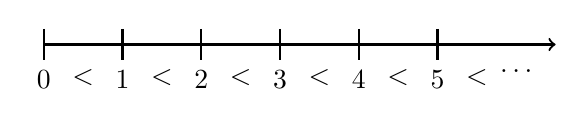
\begin{tikzpicture}
		\draw[->, thick] (0,0) -- (6.5,0);
		\foreach \x in {0,1,2,3,4,5}
			\draw[thick] (\x, 0.2) -- (\x, -0.2) node[below] {$\x$};
	
		\path (6, -0.2) node[below, text=black] {$\dots $};
			
		\foreach \x in {0,1,2,3,4,5}
			\path (\x + 0.5, -0.2) node[below, text=black] {$<$};
	\end{tikzpicture}
\end{figure}

\example

Пусть $X$ --- множество аудиторий корпуса некоторого университета, $x, y \in X$. Пусть $\boxed{x \succ y}$, если аудитория $x$ находится на более высоком этаже, чем аудитория $y$.

Это отношение является отношением частичного строгого порядка, потому что сравнить между собой можно лишь аудитории на разных этажах. Значит на множестве $X$ есть несравнимые элементы --- аудитории на одном этаже. Максимальными аудиториями будут те, которые находятся на самом высоком этаже.

\algorithm[процесс принятия решений с переменным числом шагов]\label{alg:unknown_step_process}

\textbf{Общие соображения}

В \hyperref[alg:n_step_process]{$N$-шаговом процессе принятия решений} у нас были состояния и решения на каждом шаге, начальное состояние, фиксированное число шагов, функция перехода и целевая функция, значение которой нужно оптимизировать. Теперь у нас всё то же самое, но количество шагов заранее неизвестно. Возникает вопрос: а как понять, сколько шагов совершить, то есть в какой момент остановить алгоритм?

Пусть $P$ --- множество возможных состояний, на котором определено отношение частичного строгого порядка $\succ$. Определим \underline{условие остановки} следующим образом: алгоритм останавливается, если текущее состояние $p$ принадлежит множеству конечных состояний $\bar{P}$. Определим $\bar{P}$ как множество максимальных элементов множества $P$ в смысле отношения $\succ$, то есть
\[
\bar{P} = \big\{x \in P \ \big| \ \forall y \in P: x \nsucc y\big\}.
\]

Итого, нам известно множество возможных состояний $P$, начальное состояние $p_0$ и множество конечных состояний $\bar{P} \subseteq P$, тогда мы получаем задачу поиска пути $(p^*_1 = p_0, p^*_2, p^*_3, \cdots, p^*_k)$, который даст оптимальное значение целевой функции исходной задачи (например, минимальные затраты), при этом $p^*_k \in \bar{P}$ и все переходы осуществимы, то есть $p^*_{i+1} = T(p^*_{i}, q)$. Заметим, что в таком случае количество шагов, которое нужно будет совершить, равняется $k$.

Для корректности алгоритма необходимо на множестве $P$ определить правила того, как можно перемещаться между состояниями в соответствии с задачей, иначе мы сможем ходить циклами, строя неоптимальные маршруты, а оптимальный так и не получим. Для этого необходимо, чтобы функция перехода $T(p, q)$ была <<согласована>> с отношением $\succ$ на множестве $P$, то есть чтобы
\[
\forall p \in P \quad T(p, q) \succ p.
\]

Выполнимость этого гарантирует, что какие бы решения мы не принимали, мы сможем попасть в конечное состояние.

\begin{figure}[H]
	\centering
	\begin{tikzpicture}[
		arrow/.style={-Stealth, thick, shorten >= 2pt, shorten <= 2pt}
		]
		
		% Рисуем главный овал и заливаем его светло-синим
		\draw[fill=blue!15, draw=blue, thick] (0,0) ellipse (2cm and 3cm);
		
		% Рисуем границу, разделяющую овал на P и ~P
		\draw[thick] (1.5, 2) .. controls (1, 1) and (1, -1) .. (1.5, -2);
		
		% Подписываем множество P (слева от разделителя)
		\node at (-1.5, 0.5) {\Large $P$};
		
		% Подписываем множество ~P (справа от разделителя)
		\node at (1.5, 0.5) {\Large $\bar{P}$};
		
		% Определяем точки p_0, p_1, p_2 в множестве P
		\coordinate (p0) at (-0.5, 1.8);
		\coordinate (p1) at (-1.0, 0);
		\coordinate (p2) at (-0.2, -1.4);
		\coordinate (p3) at (0.4, 0);
		\coordinate (pk) at (1.8, 0);
		
		% Рисуем точки и подписываем их
		\fill[red] (p0) circle (2pt) node[above left] {$p_0$};
		\fill[red] (p1) circle (2pt) node[below left] {$p_1$};
		\fill[red] (p2) circle (2pt) node[below left] {$p_2$};
		\fill[red] (p3) circle (2pt) node[above left] {$p_3$};
		\fill[red] (pk) circle (2pt) node[below left] {$p_k$};
		
		% Рисуем стрелки из конкретных точек p_i в множество ~P
		\draw[arrow, red] (p0) to [bend left=15] (p1);
		\draw[arrow, red] (p1) to [bend left=10] (p2);
		\draw[arrow, red] (p2) to [bend left=-15] (p3);
		\draw[arrow, red] (p3) to (pk);
		
	\end{tikzpicture}
	\caption{Пример пути из $p_0$ в $p_k$ ($k=4$)}
\end{figure}

\textbf{Подход к выбору оптимальной стратегии}

В \hyperref[alg:n_step_process]{$N$-шаговом процессе принятия решений} мы рассматривали семейства задач $(n, p)$ и строили оптимальную стратегию, идя от $n = N$ к $n = 1$ и минимизируя значение функции дохода $g_n(p, q)$. При этом мы шли от состояний, которые были на шаге $n=N$, к начальному состоянию на шаге $n=1$ (<<обратный ход>>). Здесь мы также будем на каждом шаге оптимизировать функцию дохода $g(p, q)$, но идти будем от конечных состояний к начальному.

\begin{figure}[H]
	\centering
	\begin{tikzpicture}[
		arrow/.style={-Stealth, thick, shorten >= 2pt, shorten <= 2pt}
		]
		
		% Рисуем главный овал и заливаем его светло-синим
		\draw[fill=blue!15, draw=blue, thick] (0,0) ellipse (2cm and 3cm);
		
		% Рисуем границу, разделяющую овал на P и ~P
		\draw[thick] (1.5, 2) .. controls (1, 1) and (1, -1) .. (1.5, -2);
		
		% Подписываем множество P (слева от разделителя)
		\node at (-1.5, 0.5) {\Large $P$};
		
		% Подписываем множество ~P (справа от разделителя)
		\node at (1.5, 0.5) {\Large $\bar{P}$};
		
		% Определяем точки p_0, p_1, p_2 в множестве P
		\coordinate (p0) at (-0.5, 1.8);
		\coordinate (p1) at (-1.0, 0);
		\coordinate (p2) at (-0.2, -1.4);
		\coordinate (p3) at (0.4, 0);
		\coordinate (pk) at (1.8, 0);
		
		% Рисуем точки и подписываем их
		\fill[red] (p0) circle (2pt) node[above left] {$p_0$};
		\fill[red] (p1) circle (2pt) node[below left] {$p_1$};
		\fill[red] (p2) circle (2pt) node[below left] {$p_2$};
		\fill[red] (p3) circle (2pt) node[above left] {$p_3$};
		\fill[red] (pk) circle (2pt) node[below left] {$p_k$};
		
		% Рисуем стрелки из конкретных точек p_i в множество ~P
		\draw[arrow, red] (p1) to [bend left=15] (p0);
		\draw[arrow, red] (p2) to [bend left=10] (p1);
		\draw[arrow, red] (p3) to [bend left=-15] (p2);
		\draw[arrow, red] (pk) to (p3);
		
	\end{tikzpicture}
	\caption{Пример <<обратного хода>> из $p_k$ в $p_0$ ($k=4$)}
\end{figure}

Для этого на каждом шаге будем определять текущее \underline{множество конечных состояний}. На самом первом шаге это множество $\bar{P}_0 = \bar{P}$ (из условия), на втором шаге это $\bar{P}_1 = \max(P \setminus \bar{P}_0)$, на третьем шаге это $\bar{P}_2 = \max(P \setminus \bar{P}_0 \setminus \bar{P}_1)$ и так далее, где $\max(A)$ --- множество максимальных элементов множества $A$. Данный выбор множеств конечных состояний обусловлен следующим: для завершения процесса нам нужно оказаться в состоянии из множества $\bar{P}$, оказаться в состоянии из этого множества за один шаг можно, если находимся в состоянии из $\bar{P}_1$; оказаться в состоянии из $\bar{P}_1$ можно за один шаг, если находимся в состоянии из $\bar{P}_2$ и так далее. Таким образом, получается цепочка переходов между множествами конечных состояний
\[
\bar{P}_k \to \bar{P}_{k-1} \to \dots \to \bar{P}_3 \to \bar{P}_2 \to \bar{P}_1 \to \bar{P}_0 = \bar{P},
\]

при этом $p_o \in \bar{P}_k$ и каждый переход осуществим за шаг.

\begin{figure}[H]
	\centering
	\begin{tikzpicture}[
		arrow/.style={-Stealth, thick, shorten >= 2pt, shorten <= 2pt},
		cross/.style={black, thick, rotate=0}
		]
		
		% Рисуем главный овал и заливаем его светло-синим
		\draw[fill=blue!15, draw=blue, thick] (0,0) ellipse (2cm and 3cm);
		
		% Рисуем границу, разделяющую овал на P и ~P
		\draw[thick] (1.5, 2) .. controls (1, 1) and (1, -1) .. (1.5, -2);
		
		% Подписываем множество P (слева от разделителя)
		\node at (-1.5, 0.5) {\Large $P$};
		
		% Подписываем множество ~P (справа от разделителя)
		\node at (1.5, 0.5) {\Large $\bar{P}$};
		
		\node at (0.6, -2) {\Large $\bar{P_1}$};
		
		\draw[thick] (1.15, 0) .. controls (0, 0) and (0.2, -1) .. (0, -3);
		
		\draw[cross] (1.3, 1.0) -- (1.7, 1.4);
		\draw[cross] (1.3, 1.4) -- (1.7, 1.0);
		
		\draw[cross] (1.3, 0.1) -- (1.7, -0.3);
		\draw[cross] (1.3, -0.3) -- (1.7, 0.1);
		
		\draw[cross] (1.3, -0.4) -- (1.7, -0.8);
		\draw[cross] (1.3, -0.8) -- (1.7, -0.4);
		
		\draw[cross] (1.3, -1) -- (1.7, -1.4);
		\draw[cross] (1.3, -1.4) -- (1.7, -1);
		
		\draw[arrow, red, very thick] (0.6, -1) to [bend left=-15] (1.5, 0);
		\draw[arrow, red, very thick] (0.6, -1.4) to [bend left=-15] (1.5, -0.4);
	\end{tikzpicture}
	\caption{Иллюстрация множеств конечных состояний}
\end{figure}

По аналогии с \hyperref[alg:opt_strategy]{алгоритмом выбора оптимальной стратегии $N$-шагового процесса} введём функцию $f(p)$ (теперь она не имеет индекса, поскольку нет конкретным шагов). Эта функция будет обозначать оптимальное значение целевой функции исходной задачи, если мы находимся в состоянии $p$. Фактически эта функция показывает оптимальное значение целевой функции при некотором оптимальном пути из состояния $p$ в множество конечных состояний $\bar{P}$. Как и в алгоритме выбора оптимальной стратегии $N$-шагового процесса, для каждого состояния $p$ будем рассчитывать и запоминать значение $f(p)$ вместе с оптимальным решением.

\bigskip

\textbf{Алгоритм}

Для осуществления алгоритма нужны следующие \underline{исходные данные}

\begin{itemize}[nosep]
	\item \definitionfont{состояние} на каждом шаге. Обозначение: $\boxed{p}$;
	
	\item \definitionfont{множество возможных состояний}, на котором определено отношение частичного строгого порядка $\succ$. Обозначение: $\boxed{P} = \{p_0, p_1, p_2, \dots\}$;
	
	\item \definitionfont{начальное состояние}. Обозначение: $\boxed{p_0}$;
	
	\item \definitionfont{множества конечных состояний}
	\[
	\bar{P}_0 = \bar{P},
	\]
	\[
	\forall k > 0 \quad \bar{P}_k = \max(P \setminus \bar{P}_0 \setminus \bar{P}_1 \dots \setminus \bar{P}_{k-1});
	\]

	\item \definitionfont{решение} на каждом шаге. Обозначение: $\boxed{q}$;
	
	\item \definitionfont{множество возможных решений}. Обозначение $\boxed{Q}$;
	
	\item \definitionfont{функция перехода} --- функция перехода из текущего состояния $p$ в новое состояние $p'$, если принимается решение $q$. Обозначение: $\boxed{T(p, q)}$.
	\[
	p' = T(p, q),
	\]
	\[
	\forall p \in P \quad \underbrace{T(p, q) \succ p}_{\text{<<согласованность>>}}
	\]
	
	\item \definitionfont{множество допустимых решений} в состоянии $p$. Обозначение: $\boxed{Q(p)}$;
	
	\item \definitionfont{функция дохода} --- оптимальное значение целевой функции на одном шаге, если в состоянии $p$ принимается решение $q$. Обозначение: $\boxed{g(p, q)}$;
	
	\item $\boxed{f(p)}$ --- оптимальное значение целевой функции, если вначале было состояние $p$.
\end{itemize}

\bigskip

\underline{Рекуррентные соотношения}

\[
\forall p \in \bar{P} \quad f(p) = 0,
\]
\[
\forall p \notin \bar{P} \quad f(p) = \min_{q \in Q(p)} \Big\{ g(p, q) + f\big(T(p, q)\big) \Big\}.
\]

\begin{note}
	Значение $f(p)$ для конечного состоянии $p$ определяется конкретной задачей. Так, если в задаче на всех шагах предполагается суммирование (как в \hyperref[pr:car_on_island]{задаче о машине}), то $f(p) = 0$, а если в задаче предполагается умножение (как в  \hyperref[pr:rockets]{задаче о ракетах}), то $f(p) = 1$ и так далее.
\end{note}

\begin{note}
	В общем случае $f(p)$ может записываться не только с помощью $\min$, но и с помощью $\max$. Также операция между $g(p, q)$ и $f\big(T(p, q)\big)$ может быть как сложение, так и умножение, взятие минимума/максимума и так далее.
\end{note}

\bigskip

\underline{Алгоритм}

Все промежуточные результаты по аналогии с \hyperref[alg:opt_strategy]{алгоритмом выбора оптимальной стратегии принятия решений} будут фиксироваться в следующей таблице

\begin{table}[H]
	\centering
	\begin{tabular}{ | c | c | } 
		\hline
		$p$ & $(f, q)$ \\ 
		\hline
		$p_0$ & \\\hline
		$p_1$ & \\\hline
		$p_2$ & \\\hline
		$\dots$ & \\\hline
	\end{tabular}
\end{table}

Сначала на каждом шаге считаем значения $f(p)$ для $p$ из текущего множества конечных состояний и фиксируем в таблице значение $f(p)$ и решение, на котором достигается оптимальное значение целевой функции --- <<обратный ход>>.

После того, как таблица заполнена, будем выбирать оптимальную стратегию --- <<прямой ход>>. Делать это будем следующим образом

\begin{align*}
	p_1^* = p_0&, \qquad &q_1^* = q(p_1^*), \\
	p_2^* = T(p_1^*, q_1^*)&, &q_2^* = q(p_2^*), \\
	p_3^* = T(p_2^*, q_2^*)&, &q_3^* = q(p_3^*), \\
	\dots& &\dots \\
	p_k^* = T(p_{k-1}^*, q_{k-1}^*)&, &q_k^* = q(p_k^*), \\
	p_{k+1}^* = T(p_{k}^*, q_{k}^*) \in \bar{P}&.
\end{align*}

Заметим, что мы закончили в тот момент, когда очередное состояние $p^*_{k+1}$ оказалось конечным.

По итогам <<прямого хода>> получим стратегию $q^* = \{q_1^*, q_2^*, \dots, q^*_{k-1}, q^*_k\}$, при этом количество шагов $k$ определяется именно в этот момент.

\section{Задача о дороге}

\problem[о дороге]\label{pr:road}

Дорога состоит из 8 последовательных участков. Для поддержания её в нормальном состоянии решено разместить вдоль дороги дорожно-ремонтные станции. Известно что затраты на обслуживание участка от $x$ до $y$ одной станцией составляет величину $f(x, y)$, задаваемую таблицей. Известно также, что одна станция не может обслуживать отрезок дороги, содержащий более 4 участков. Каким образом разделить дорогу между станциями, чтобы затраты на обслуживание дороги были минимальными? 

\begin{table}[H]
	\centering
	\begin{tabular}{| c | c | c | c | c | c | c | c | c | c |} 
		\hline
		\textbf{$x / y$} & $0$ & $1$ & $2$ & $3$ & $4$ & $5$ & $6$ & $7$ & $8$ \\\hline
		\textbf{$0$} & $2$ & $3$ & $5$ & $6$ & $15$ & $-$ & $-$ & $-$ & $-$ \\\hline
		\textbf{$1$} & $-$ & $2$ & $4$ & $6$ & $10$ & $12$ & $-$ & $-$ & $-$ \\\hline
		\textbf{$2$} & $-$ & $-$ & $2$ & $3$ & $7$ & $8$ & $10$ & $-$ & $-$ \\\hline
		\textbf{$3$} & $-$ & $-$ & $-$ & $2$ & $4$ & $7$ & $8$ & $15$ & $-$ \\\hline
		\textbf{$4$} & $-$ & $-$ & $-$ & $-$ & $2$ & $3$ & $6$ & $12$ & $15$ \\\hline
		\textbf{$5$} & $-$ & $-$ & $-$ & $-$ & $-$ & $2$ & $5$ & $10$ & $12$ \\\hline
		\textbf{$6$} & $-$ & $-$ & $-$ & $-$ & $-$ & $-$ & $2$ & $7$ & $10$ \\\hline
		\textbf{$7$} & $-$ & $-$ & $-$ & $-$ & $-$ & $-$ & $-$ & $2$ & $6$ \\\hline
		\textbf{$8$} & $-$ & $-$ & $-$ & $-$ & $-$ & $-$ & $-$ & $-$ & $2$ \\\hline
		
	\end{tabular}
\end{table}

\mathmodel

Эта задача является частным случаем \hyperref[pr:nearest_neighbor_problem]{задачи о ближайшем соседе}, за исключением того, что в данной задаче количество сегментов разбиения трассы не задано.

\begin{figure}[H]
	\centering
	\begin{tikzpicture}
		\def\radius{10cm}
		\def\ticklen{-3mm}
		
		\draw[red, very thick, densely dashed](-30:\radius) arc[start angle=-30, end angle=-50, radius=\radius];
		
		\draw[blue!80!black, very thick, dotted](-50:\radius) arc[start angle=-50, end angle=-70, radius=\radius];
		
		\draw[green!50!black, thick, double] (-70:\radius) arc[start angle=-70, end angle=-110, radius=\radius];
		
		\foreach \a/\txt in {
			-30/{$8$},
			-40/{$7$},
			-50/{$6$},
			-60/{$5$},
			-70/{$4$},
			-80/{$3$},
			-90/{$2$},
			-100/{$1$},
			-110/{$0$}}
		{
			\path (\a:\radius) coordinate (P);
			\fill (P) circle (2pt);			
			\node[font=\small] at ($(P)+({\a+200}:2*\ticklen)$) {\txt};
		}
	\end{tikzpicture}
	\caption{Пример разбиения трассы на 3 сегмента $(0 \to 4)$, $(4 \to 6)$, $(6 \to 8)$.}
\end{figure}

Пусть $i = 1 \dots 8$ --- точки, где можно ставить станции (в точке $i=0$ станция устанавливается по умолчанию).

\bigskip

\textit{Параметры}

\begin{itemize}[nosep]
	\item $f(x, y)$ --- затраты на обслуживания участка $(x \to y$).
\end{itemize}

\bigskip

\textit{Переменные}

\begin{itemize}[nosep]	
	\item $x = \{x_i\}$ --- точки, где нужно строить станции.
\end{itemize}

\solution

Будем решать задачу с помощью динамического программирования, однако поскольку нам неизвестно количество шагов, для решения будем использовать \hyperref[alg:unknown_step_process]{процесс принятия решений с переменным числом шагов}.

\bigskip

\textbf{Исходные данные}
\begin{itemize}[nosep]	
	\item \underline{на каждом шаге} будем определять в какой точке нужно ставить станцию обслуживания;
	
	\item \underline{состояние} на каждом шаге $(p)$ --- точка начала участка, в конце которого будет установлена станция;
	
	\item \underline{решение} на каждом шаге $(q)$ --- насколько нужно продвинуться вперёд от начала участка для установки станции;
	
	\item \underline{множество возможных состояний}
	\[P= \big\{0, 1, 2, \cdots, 8 \big\},\]
	
	на этом множестве установлен линейный строгий порядок, поскольку участки дороги следуют друг за другом;
	
	\item \underline{функция перехода} --- точка конца текущего и начала следующего участков
	\[p' = T(p, q) = p + q,\]
	
	функция перехода <<согласована>> с линейным строгим порядком на множестве $P$;
	
	\item \underline{множества конечных состояний};
	\[
	\bar{P} = \{8\}, \quad \bar{P_1} = \{7\}, \quad \bar{P_2} = \{6\},
	\]
	\[
	\bar{P_3} = \{5\}, \quad \bar{P_4} = \{4\}, \quad \bar{P_5} = \{3\},
	\]
	\[
	\bar{P_6} = \{2\}, \quad \bar{P_7} = \{1\}, \quad \bar{P_8} = \{0\};
	\]
	
	\item в рамках задачи будет удобнее работать не с $q$, а с $p'= p + q$, в связи с этим определим \underline{множество возможных значений для $p'$}
	\[P^{'} = \{1, 2, 3, 4, 5, 6, 7, 8\};\]
	
	\item \underline{множества допустимых значений для $p'$}; учтём, что одна станция может обслуживать не более 4 точек дороги, а также что в одной точке дороги не может быть больше одной станции
	\[P^{'}(p) = \{p+1, p+2, \cdots, \min(p + 4, 8)\}.\]
\end{itemize}

Для решения данной задачи будем рассматривать различные подзадачи, в каждой из которых своё множество конечных состояний $\bar{P}_k$. В рамках данной задачи это будет означать следующее: мы будем рассматривать подзадачи, в которых нам доступна не вся дорога, а лишь её часть, которая начинается в точке $p \in \bar{P}_k$ и кончается в точке 8.

\bigskip

\textbf{База процесса}

Пусть $f(p)$ --- это минимальные затраты на содержание дороги, если она начинается в точке $p$ (в таком случае считается, что в точке $p$ станция установлена), $f(0)$ --- исходная задача.

По \hyperref[alg:unknown_step_process]{теории} $f(8) = 0$ --- база процесса, которую мы будем использовать для перехода.

\begin{note}
	По таблице $f(8, 8) = 2$ --- затраты на содержание двух станций, которые будут установлены в точке $8$. В то время как $f(8)$ --- содержание лишь одной станции, установленной в точке $8$, поэтому $f(8) = 0 \neq f(8, 8) = 2$.
\end{note}

\bigskip

\textbf{Переход}

Пусть на некотором шаге у нас есть множество конечных состояний $\bar{P}_k$, тогда будем считать $f(p)$ для $p \in \bar{P}_k$ в предположении, что $f(p')$ мы знаем $\forall p' \in P^{'}(p)$. Напишем рекуррентное соотношение для $f(p)$
\[
\boxed{f(p) = \min_{p' \in P^{'}(p)} \Big\{f(p, p') + f(p') \Big\}},\tag{*}
\]

\begin{itemize}[nosep]
	\item $f(p, p')$ --- затраты на первый сегмент дороги $(p \to p')$, при этом дорога начинается в точке $p$;
	
	\item $f(p')$ --- минимальные затраты на содержание оставшейся части дороги $(p' \to 8)$; по предположению значение уже известно.
\end{itemize}

Исходя из множества возможных состояний $P$, составим таблицу.

\begin{table}[H]
	\centering
	\begin{tabular}{ | c | c | } 
		\hline
		$p$ & $(f, p')$ \\ 
		\hline
		$0$ & \\\hline
		$1$ & \\\hline
		$2$ & \\\hline
		$3$ & \\\hline
		$4$ & \\\hline
		$5$ & \\\hline
		$6$ & \\\hline
		$7$ & \\\hline
		$8$ & \\\hline
	\end{tabular}
\end{table}

Искомое значение --- это $\mathbf{f(p_0) = f(0)}$. Заполним таблицу, чтобы найти его, и определить точки где нужно ставить станции (оптимальное разбиение дороги).

\bigskip

\textbf{Заполнение таблицы}
\begin{enumerate}[nosep]
	\item[\fbox{$\bar{P}$}] Рассматриваем первое множество конечных состояний $\bar{P} = \{8\}$, то есть нам доступна лишь части дороги $(8 \to 8)$, таким образом мы можем поставить станцию лишь в точке 8.
	
	\[
	f(p) = f(8) = 0.
	\]
	
	Занесём данные в таблицу.
	
	\begin{table}[H]
		\centering
		\begin{tabular}{ | c | c |} 
			\hline
			$p$ & $(f, p')$ \\ 
			\hline
			$0$ & \\\hline
			$1$ & \\\hline
			$2$ & \\\hline
			$3$ & \\\hline
			$4$ & \\\hline
			$5$ & \\\hline
			$6$ & \\\hline
			$7$ & \\\hline
			$8$ & $(0, 0)$ \\\hline
		\end{tabular}
	\end{table}
	
	\begin{note}
		Значение $p'$ в при $p = 8$ в таблице не имеет никакого значения, поэтому можно просто оставить его нулём.
	\end{note}
	
	\item[\fbox{$\bar{P_1}$}] Рассматриваем второе множество конечных состояний $\bar{P_1} = \{7\}$, то есть нам доступна лишь часть дороги $(7 \to 8)$. Выражение для этого и последующих множеств выглядит как рекуррентное соотношение (*)
	
	\[
	f(p) = f(7) = \begin{array}{c|l}
		\underbrace{8}_{p'} & f(7,8) + f(8) = 6 + 0 = \circled{6}\\
	\end{array}
	\]
	
	Занесём данные в таблицу.
	
	\begin{table}[H]
		\centering
		\begin{tabular}{ | c | c |} 
			\hline
			$p$ & $(f, p')$ \\ 
			\hline
			$0$ & \\\hline
			$1$ & \\\hline
			$2$ & \\\hline
			$3$ & \\\hline
			$4$ & \\\hline
			$5$ & \\\hline
			$6$ & \\\hline
			$7$ & $(6, 8)$ \\\hline
			$8$ & $(0, 0)$ \\\hline
		\end{tabular}
	\end{table}
	
	\item[\fbox{$\bar{P_2}$}] Рассматриваем множество конечных состояний $\bar{P_2} = \{6\}$, то есть нам доступна лишь часть дороги $(6 \to 8)$.
	
	\[
	f(p) = f(6) = \begin{array}{c|l}
		7 & f(6,7) + f(7) = 7 + 6 = 13\\
		\underbrace{8}_{p'} & f(6,8) + f(8) = 10 + 0 = \circled{10}\\
	\end{array}
	\]
	
	Занесём данные в таблицу.
	
	\begin{table}[H]
		\centering
		\begin{tabular}{ | c | c |} 
			\hline
			$p$ & $(f, p')$ \\ 
			\hline
			$0$ & \\\hline
			$1$ & \\\hline
			$2$ & \\\hline
			$3$ & \\\hline
			$4$ & \\\hline
			$5$ & \\\hline
			$6$ & $(10, 8)$ \\\hline
			$7$ & $(6, 8)$ \\\hline
			$8$ & $(0, 0)$ \\\hline
		\end{tabular}
	\end{table}
	
	\item[\fbox{$\bar{P_3}$}] Рассматриваем множество конечных состояний $\bar{P_3} = \{5\}$.
	
	\[
	f(5) = \begin{array}{c|l}
		6 & f(5,6) + f(6) = 5 + 10 = 15\\
		7 & f(5,7) + f(7) = 10 + 6 = 16\\
		8 & f(5,8) + f(8) = 12 + 0 = \circled{12}\\
	\end{array}
	\]
	
	Занесём данные в таблицу.
	
	\begin{table}[H]
		\centering
		\begin{tabular}{ | c | c |} 
			\hline
			$p$ & $(f, p')$ \\ 
			\hline
			$0$ & \\\hline
			$1$ & \\\hline
			$2$ & \\\hline
			$3$ & \\\hline
			$4$ & \\\hline
			$5$ & $(12, 8)$ \\\hline
			$6$ & $(10, 8)$ \\\hline
			$7$ & $(6, 8)$ \\\hline
			$8$ & $(0, 0)$ \\\hline
		\end{tabular}
	\end{table}
	
	\item[\fbox{$\bar{P_4}$}] Рассматриваем множество конечных состояний $\bar{P_4} = \{4\}$.
	
	\[
	f(4) = \begin{array}{c|l}
		5 & f(4,5) + f(5) = 3 + 12 = \circled{15}\\
		6 & f(4,6) + f(6) = 6 + 10 = 16\\
		7 & f(4,7) + f(7) = 12 + 6 = 18\\
		\underbrace{8}_{p'} & f(4,8) + f(8) = 15 + 0 = \circled{15}\\
	\end{array}
	\]
	
	Занесём данные в таблицу. Учтём, что оптимальное значение целевой функции $f(p)=15$ достигается при $p' = 5$ и $p' = 8$. В таблице это будет записано как $(15, 5/8)$.
	
	\begin{table}[H]
		\centering
		\begin{tabular}{ | c | c |} 
			\hline
			$p$ & $(f, p')$ \\ 
			\hline
			$0$ & \\\hline
			$1$ & \\\hline
			$2$ & \\\hline
			$3$ & \\\hline
			$4$ & $(15, 5/8)$ \\\hline
			$5$ & $(12, 8)$ \\\hline
			$6$ & $(10, 8)$ \\\hline
			$7$ & $(6, 8)$ \\\hline
			$8$ & $(0, 0)$ \\\hline
		\end{tabular}
	\end{table}
	
	\item[\fbox{$\bar{P_5}$}] Рассматриваем множество конечных состояний $\bar{P_5} = \{3\}$.
	
	\[
	f(3) = \begin{array}{c|l}
		4 & f(3,4) + f(4) = 4 + 15 = 19\\
		5 & f(3,5) + f(5) = 7 + 12 = 19\\
		6 & f(3,6) + f(6) = 8 + 10 = \circled{18}\\
		\underbrace{7}_{p'} & f(3,7) + f(7) = 15 + 6 = 21\\
	\end{array}
	\]
	
	Занесём данные в таблицу.
	
	\begin{table}[H]
		\centering
		\begin{tabular}{ | c | c |} 
			\hline
			$p$ & $(f, p')$ \\ 
			\hline
			$0$ & \\\hline
			$1$ & \\\hline
			$2$ & \\\hline
			$3$ & $(18, 6)$ \\\hline
			$4$ & $(15, 5/8)$ \\\hline
			$5$ & $(12, 8)$ \\\hline
			$6$ & $(10, 8)$ \\\hline
			$7$ & $(6, 8)$ \\\hline
			$8$ & $(0, 0)$ \\\hline
		\end{tabular}
	\end{table}
	
	\item[\fbox{$\bar{P_6}$}] Рассматриваем множество конечных состояний $\bar{P_6} = \{2\}$.
	
	\[
	f(2) = \begin{array}{c|l}
		3 & f(2,3) + f(3) = 3 + 18 = 21\\
		4 & f(2,4) + f(4) = 7 + 15 = 22\\
		5 & f(2,5) + f(5) = 8 + 12 = \circled{20}\\
		\underbrace{6}_{p'} & f(2,6) + f(6) = 10 + 10 = \circled{20}\
	\end{array}
	\]
	
	Занесём данные в таблицу. Учтём, что оптимальное значение целевой функции $f(p)=20$ достигается при $p' = 5$ и $p' = 6$. В таблице это будет записано как $(20, 5/6)$.
	
	\begin{table}[H]
		\centering
		\begin{tabular}{ | c | c |} 
			\hline
			$p$ & $(f, p')$ \\ 
			\hline
			$0$ & \\\hline
			$1$ & \\\hline
			$2$ & $(20, 5/6)$ \\\hline
			$3$ & $(18, 6)$ \\\hline
			$4$ & $(15, 5/8)$ \\\hline
			$5$ & $(12, 8)$ \\\hline
			$6$ & $(10, 8)$ \\\hline
			$7$ & $(6, 8)$ \\\hline
			$8$ & $(0, 0)$ \\\hline
		\end{tabular}
	\end{table}
	
	\item[\fbox{$\bar{P_7}$}] Рассматриваем множество конечных состояний $\bar{P_7} = \{1\}$.
	
	\[
	f(1) = \begin{array}{c|l}
		2 & f(1,2) + f(2) = 4 + 20 = \circled{24}\\
		3 & f(1,3) + f(3) = 6 + 18 = \circled{24}\\
		4 & f(1,4) + f(4) = 10 + 15 = 31\\
		\underbrace{5}_{p'} & f(1,5) + f(5) = 12 + 12 = \circled{24}\
	\end{array}
	\]
	
	Занесём данные в таблицу. Учтём, что оптимальное значение целевой функции $f(p)=24$ достигается при $p' = 2$, $p'=3$ и $p' = 5$. В таблице это будет записано как $(24, 2/3/5)$.
	
	\begin{table}[H]
		\centering
		\begin{tabular}{ | c | c |} 
			\hline
			$p$ & $(f, p')$ \\ 
			\hline
			$0$ & \\\hline
			$1$ & $(24, 2/3/5)$ \\\hline
			$2$ & $(20, 5/6)$ \\\hline
			$3$ & $(18, 6)$ \\\hline
			$4$ & $(15, 5/8)$ \\\hline
			$5$ & $(12, 8)$ \\\hline
			$6$ & $(10, 8)$ \\\hline
			$7$ & $(6, 8)$ \\\hline
			$8$ & $(0, 0)$ \\\hline
		\end{tabular}
	\end{table}
	
	\item[\fbox{$\bar{P_8}$}] Рассматриваем множество конечных состояний $\bar{P_8} = \{8\}$, оно содержит $p_0$, значит сейчас нам доступна вся дорога $(0 \to 8)$, таким образом это последнее множество конечных состояний, которое нам нужно рассмотреть.
	
	значит оно последнее, которое нам нужно рассмотреть.
	
	\[
	f(0) = \begin{array}{c|l}
		1 & f(0,1) + f(1) = 3 + 24 = 27\\
		2 & f(0,2) + f(2) = 5 + 20 = \circled{25}\\
		3 & f(0,3) + f(3) = 8 + 18 = 26\\
		\underbrace{4}_{p'} & f(0,4) + f(4) = 15 + 15 = 30\
	\end{array}
	\]
	
	Занесём данные в таблицу.
	
	\begin{table}[H]
		\centering
		\begin{tabular}{ | c | c |} 
			\hline
			$p$ & $(f, p')$ \\ 
			\hline
			$0$ & $(25, 2)$ \\\hline
			$1$ & $(24, 2/3/5)$ \\\hline
			$2$ & $(20, 5/6)$ \\\hline
			$3$ & $(18, 6)$ \\\hline
			$4$ & $(15, 5/8)$ \\\hline
			$5$ & $(12, 8)$ \\\hline
			$6$ & $(10, 8)$ \\\hline
			$7$ & $(6, 8)$ \\\hline
			$8$ & $(0, 0)$ \\\hline
		\end{tabular}
	\end{table}
	
	\bigskip
	
	\textbf{Поиск оптимальной стратегии}
	
	Наше начальное состояние $p_0 = 0$, поскольку первый участок начинается в точке 0.
	\begin{alignat*}{2}
		p_1^* = p_0 = 0 &, \qquad\qquad &&p_1^{'*} = 2, \\
		p_2^* = p_1^{'*} = 2 &, &&p_2^{'*} = 5, \\
		p_3^* =p_2^{'*} = 5 &, &&p_3^{'*} = 8 \in \bar{P}.
	\end{alignat*}
	
	Итоговая стратегия --- это $p^{'*} = \{2, 5, 8\}$, то есть станции нужно ставить в точках $2$, $5$ и $8$, в таком случае затраты на содержание дороги составят $f(0)=25$. Таким образом, в ходе решения задачи выяснилось, что для минимизации расходов нужно строить 3 станции.
	
	\begin{note}
		$p_2^{'*}$ можно было выбрать равным 6, это бы привело к стратегии $p^{'*} = \{2, 6, 8\}$, но затраты остались бы такими же.
	\end{note}
\end{enumerate}

\section{Задача о моторах}

\problem[о моторах]

Имеется потребность в моторах 8 типов. Моторы $i$-го типа требуются в количестве $a_i$ штук. Известно, что мотор $i$-го типа можно заменить мотором $k$-го типа, если $i < k$. Завод может производить не более трёх типов моторов. Стоимость производства одного мотора $i$-го типа равняется $30 u_i$, а затраты на организацию производства моторов этого типа составляет $600 + 50 u_i$. Какие типы моторов и в каких количествах следует производить на заводе, чтобы полностью удовлетворить потребность в моторах всех типов. Числовые значения величин $a_i$ и $u_i$ содержатся в таблице.

\begin{table}[H]
	\centering
	\begin{tabular}{ | c | c | c | c | c | c | c | c | c | } 
		\hline
		$i$ & $1$ & $2$ & $3$ & $4$ & $5$ & $6$ & $7$ & $8$\\\hline
		$a_i$ & $50$ & $20$ & $40$ & $80$ & $20$ & $50$ & $10$ & $20$\\\hline
		$u_i$ & $0.3$ & $0.4$ & $0.5$ & $0.6$ & $0.7$ & $0.8$ & $0.9$ & $1$\\\hline
	\end{tabular}
\end{table}

\mathmodel

Сведём задачу к \hyperref[pr:nearest_neighbor_problem]{задаче о ближайшем соседе}. Для этого нужно определить точки нашей трассы, количество точек разбиения и функцию расстояния. Пусть точки нашей трассы --- это типы моторов, а функция расстояния --- это затраты на производство моторов в нужных количествах.

В \hyperref[pr:road]{задаче о дороге} мы разбивали трассу на участки, при этом в конце и в начале каждого участка устанавливалась станция. В данной задаче мы также будем разбивать дорогу на участки, но смысл будет следующий: если в разбиении дороги присутствует участок $(x \to y)$, то заводу нужно производить моторы типов $x$ и $y$, а моторы промежуточных типов --- не нужно (потребность в них будет закрыта моторами типа $y$). Таким образом, нужно найти разбиение трассы, состоящей из типов моторов, на участки.

\begin{figure}[H]
	\centering
	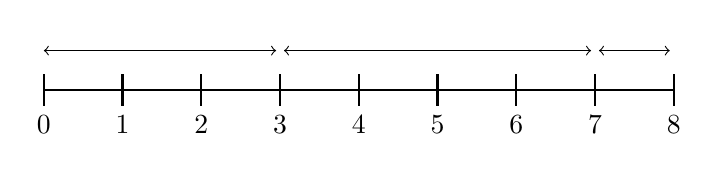
\begin{tikzpicture}		
		\draw[thick] (0,0) -- (8,0);
		\foreach \x in {0,1,2,3,4,5, 6, 7, 8}
			\draw[thick] (\x, 0.2) -- (\x, -0.2) node[below] {$\x$};
		\draw [<->] (0, 0.5) -- node[above=0.5mm] {$$} (2.95, 0.5);
		\draw [<->] (3.05, 0.5) -- node[above=0.5mm] {$$} (6.95, 0.5);
		\draw [<->] (7.05, 0.5) -- node[above=0.5mm] {$$} (7.95, 0.5);
		
	\end{tikzpicture}
	\caption{Пример разбиение трассы в данной задаче на три участка: $(0 \to 3)$, $(3 \to 7)$, $(7 \to 8)$. Это означает, что заводу нужно производить моторы 3-го, 7-го и 8-го видов.}
\end{figure}

Итак, $Z = \{0, 1, 2, \dots, 7, 8\}$ --- точки трассы. Моторов нулевого типа нет, поэтому точка 0 является фиктивной (смысл её добавления в трассу будет объяснён далее).

Теперь нужно определить функцию расстояния $f(x, y)$. Эта функция будет иметь следующий смысл: это затраты на производство моторов типа $y$ <<в нужных количествах>>. Фраза <<в нужных количествах>> означает, что сюда вкладывается как удовлетворение потребностей как непосредственно в моторах типа $y$, так и в моторах меньшего типа. Например, если у нас есть участок $(3 \to 8)$, то в $f(3, 8)$ будут учтены затраты на производство моторов 8-го типа так, чтобы закрыть потребности в моторах 4-го, 5-го, 6-го, 7-го и 8-го типов.

Исходя из условия задачи, запишем выражение для $f(x, y)$
\[
f(x, y) = 600 + 50 \cdot u_y + 30 \cdot u_y \cdot (a_{x+1} + a_{x+2} + \dots + a_{y-1} + a_y).
\]

\begin{itemize}[nosep]
	\item $600 + 50 \cdot u_y$ --- настройка оборудования для производства моторов типа $y$;
	
	\item $30 \cdot u_y \cdot (a_{x+1} + a_{x+2} + \dots + a_{y-1} + a_y)$ --- закрытие потребностей в моторах типа $y$.
\end{itemize}

Заметим, что если бы во множество точек трассы не входил ноль, то пришлось бы отдельно расписывать $f(1, y)$, поэтому добавление нуля во множество точек трассы позволяет обобщить выражение для $f(x, y)$ на все случаи. Можно считать, что моторы 0-го типа есть и по умолчанию производятся в нужных количествах, однако закрыть потребность в других с их помощью нельзя.

В условии задачи сказано, что завод может производить моторы не более трёх типов, то есть завод может производить моторы одного типа, двух и трёх. Если бы было сказано, что завод может производить ровно $N$ типов моторов, то мы бы решали задачи с помощью \hyperref[alg:n_step_process]{$N$-шагового процесса принятия решений}, однако поскольку этого не сказано, и оптимальная стратегия завода может включать производство моторов одного типа, двух и трёх, то будем решать задачу с помощью \hyperref[alg:unknown_step_process]{процесса принятия решений с переменным числом шагов}.

\solution

Пусть $f(p)$ --- минимальные затраты для закрытия потребностей во всех типах моторов, если завод может производить моторы типов $p+1$, $p+2$, $\dots$, $8$; $f(0)$ --- ответ к исходной задаче.

\bigskip

\textbf{База процесса}

\[
f(8) = 0
\]

\bigskip

\textbf{Переход}

Пусть $p \notin \bar{P}$, тогда
\[
\boxed{f(p) = \min_{p' \in P^{'}(p)} \Big\{f(p, p') + f(p') \Big\}},\tag{*}
\]

\textbf{Заполнение таблицы}

\begin{enumerate}[nosep]
	\item[$\boxed{\bar{P}_0}$]
	
	Занесём данные в таблицу.
	
	\begin{table}[H]
		\centering
		\begin{tabular}{ | c | c |} 
			\hline
			$p$ & $(f, p')$ \\ 
			\hline
			$0$ & \\\hline
			$1$ & \\\hline
			$2$ & \\\hline
			$3$ & \\\hline
			$4$ & \\\hline
			$5$ & \\\hline
			$6$ & \\\hline
			$7$ & \\\hline
			$8$ & $(0, 0)$ \\\hline
		\end{tabular}
	\end{table}
	
	\begin{note}
		Значение $p'$ в при $p = 8$ в таблице не имеет никакого значения, поэтому можно просто оставить его нулём.
	\end{note}
	
	\item[$\boxed{\bar{P}_1}$]
	
	\[
	f(7) = \begin{array}{c|l}
		\underbrace{8}_{p'} & f(7,8) + f(8) = 1250 + 0 = \circled{1250}
	\end{array}
	\]
	
	Занесём данные в таблицу.
	
	\begin{table}[H]
		\centering
		\begin{tabular}{ | c | c |} 
			\hline
			$p$ & $(f, p')$ \\ 
			\hline
			$0$ & \\\hline
			$1$ & \\\hline
			$2$ & \\\hline
			$3$ & \\\hline
			$4$ & \\\hline
			$5$ & \\\hline
			$6$ & \\\hline
			$7$ & $(1250, 8)$ \\\hline
			$8$ & $(0, 0)$ \\\hline
		\end{tabular}
	\end{table}
	
	\item[$\boxed{\bar{P}_2}$]
	
	\[
	f(6) = \begin{array}{c|l}
		7 & f(6,7) + f(7) = 915 + 1250 = 2165\\
		\underbrace{8}_{p'} & f(6,8) + f(8) = 1550 + 0 = \circled{1550}
	\end{array}
	\]
	
	Занесём данные в таблицу.
	
	\begin{table}[H]
		\centering
		\begin{tabular}{ | c | c |} 
			\hline
			$p$ & $(f, p')$ \\ 
			\hline
			$0$ & \\\hline
			$1$ & \\\hline
			$2$ & \\\hline
			$3$ & \\\hline
			$4$ & \\\hline
			$5$ & \\\hline
			$6$ & $(1550, 8)$ \\\hline
			$7$ & $(1250, 8)$ \\\hline
			$8$ & $(0, 0)$ \\\hline
		\end{tabular}
	\end{table}
	
	\item[$\boxed{\bar{P}_3}$]
	
	\[
	f(5) = \begin{array}{c|l}
		6 & f(5,6) + f(6) = 1840 + 1550 = 3390\\
		7 & f(5,7) + f(7) = 2265 + 1250 = 3515\\
		\underbrace{8}_{p'} & f(5,8) + f(8) = 3050 + 0 = \circled{3050}
	\end{array}
	\]
	
	Занесём данные в таблицу.
	
	\begin{table}[H]
		\centering
		\begin{tabular}{ | c | c |} 
			\hline
			$p$ & $(f, p')$ \\ 
			\hline
			$0$ & \\\hline
			$1$ & \\\hline
			$2$ & \\\hline
			$3$ & \\\hline
			$4$ & \\\hline
			$5$ & $(3050, 8)$ \\\hline
			$6$ & $(1550, 8)$ \\\hline
			$7$ & $(1250, 8)$ \\\hline
			$8$ & $(0, 0)$ \\\hline
		\end{tabular}
	\end{table}
	
	\item[$\boxed{\bar{P}_4}$]
	
	\[
	f(4) = \begin{array}{c|l}
		5 & f(4,5) + f(5) = 1055 + 3050 = 4105\\
		6 & f(4,6) + f(6) = 2320 + 1550 = 3870\\
		7 & f(4,7) + f(7) = 2805 + 1250 = 4055\\
		\underbrace{8}_{p'} & f(4,8) + f(8) = 3650 + 0 = \circled{3650}
	\end{array}
	\]
	
	Занесём данные в таблицу.
	
	\begin{table}[H]
		\centering
		\begin{tabular}{ | c | c |} 
			\hline
			$p$ & $(f, p')$ \\ 
			\hline
			$0$ & \\\hline
			$1$ & \\\hline
			$2$ & \\\hline
			$3$ & \\\hline
			$4$ & $(3650, 8)$ \\\hline
			$5$ & $(3050, 8)$ \\\hline
			$6$ & $(1550, 8)$ \\\hline
			$7$ & $(1250, 8)$ \\\hline
			$8$ & $(0, 0)$ \\\hline
		\end{tabular}
	\end{table}
	
	\item[$\boxed{\bar{P}_5}$]
	
	\[
	f(3) = \begin{array}{c|l}
		4 & f(3,4) + f(4) = 2070 + 3650 = \circled{5720}\\
		5 & f(3,5) + f(5) = 2735 + 3050 = 5785\\
		6 & f(3,6) + f(6) = 4240 + 1550 = 5790\\
		7 & f(3,7) + f(7) = 4265 + 1250 = 6215\\
		\underbrace{8}_{p'} & f(3,8) + f(8) = 6050 + 0 = 6050
	\end{array}
	\]
	
	Занесём данные в таблицу.
	
	\begin{table}[H]
		\centering
		\begin{tabular}{ | c | c |} 
			\hline
			$p$ & $(f, p')$ \\ 
			\hline
			$0$ & \\\hline
			$1$ & \\\hline
			$2$ & \\\hline
			$3$ & $(5720, 4)$ \\\hline
			$4$ & $(3650, 8)$ \\\hline
			$5$ & $(3050, 8)$ \\\hline
			$6$ & $(1550, 8)$ \\\hline
			$7$ & $(1250, 8)$ \\\hline
			$8$ & $(0, 0)$ \\\hline
		\end{tabular}
	\end{table}
	
	\item[$\boxed{\bar{P}_6}$]
	
	\[
	f(2) = \begin{array}{c|l}
		3 & f(2,3) + f(3) = 1225 + 5720 = 6945\\
		4 & f(2,4) + f(4) = 2790 + 3650 = \circled{6440}\\
		5 & f(2,5) + f(5) = 3575 + 3050 = 6625\\
		6 & f(2,6) + f(6) = 5200 + 1550 = 6750\\
		7 & f(2,7) + f(7) = 6045 + 1250 = 7295\\
		\underbrace{8}_{p'} & f(2,8) + f(8) = 7250 + 0 = 7250
	\end{array}
	\]
	
	Занесём данные в таблицу.
	
	\begin{table}[H]
		\centering
		\begin{tabular}{ | c | c |} 
			\hline
			$p$ & $(f, p')$ \\ 
			\hline
			$0$ & \\\hline
			$1$ & \\\hline
			$2$ & $(6440, 4)$ \\\hline
			$3$ & $(5720, 4)$ \\\hline
			$4$ & $(3650, 8)$ \\\hline
			$5$ & $(3050, 8)$ \\\hline
			$6$ & $(1550, 8)$ \\\hline
			$7$ & $(1250, 8)$ \\\hline
			$8$ & $(0, 0)$ \\\hline
		\end{tabular}
	\end{table}
	
	\item[$\boxed{\bar{P}_7}$]
	
	\[
	f(1) = \begin{array}{c|l}
		2 & f(1,2) + f(2) = 860 + 6440 = 7300\\
		3 & f(2,3) + f(3) = 1525 + 5720 = 7245\\
		4 & f(2,4) + f(4) = 3150 + 3650 = \circled{6800}\\
		5 & f(2,5) + f(5) = 3995 + 3050 = 7045\\
		6 & f(2,6) + f(6) = 5680 + 1550 = 7230\\
		7 & f(2,7) + f(7) = 6585 + 1250 = 7835\\
		\underbrace{8}_{p'} & f(1,8) + f(8) = 7850 + 0 = 7850
	\end{array}
	\]
	
	Занесём данные в таблицу.
	
	\begin{table}[H]
		\centering
		\begin{tabular}{ | c | c |} 
			\hline
			$p$ & $(f, p')$ \\ 
			\hline
			$0$ & \\\hline
			$1$ & $(6800, 4)$ \\\hline
			$2$ & $(6440, 4)$ \\\hline
			$3$ & $(5720, 4)$ \\\hline
			$4$ & $(3650, 8)$ \\\hline
			$5$ & $(3050, 8)$ \\\hline
			$6$ & $(1550, 8)$ \\\hline
			$7$ & $(1250, 8)$ \\\hline
			$8$ & $(0, 0)$ \\\hline
		\end{tabular}
	\end{table}
	
	\item[$\boxed{\bar{P}_8}$]
	
	\[
	f(0) = \begin{array}{c|l}
		1 & f(0,1) + f(1) = 1065 + 6800 = 7865\\
		2 & f(0,2) + f(2) = 1460 + 6440 = 7900\\
		3 & f(0,3) + f(3) = 2275 + 5720 = 7995\\
		4 & f(0,4) + f(4) = 4050 + 3650 = \circled{7700}\\
		5 & f(0,5) + f(5) = 5045 + 3050 = 8095\\
		6 & f(0,6) + f(6) = 6800 + 1550 = 8450\\
		7 & f(0,7) + f(7) = 7935 + 1250 = 9185\\
		\underbrace{8}_{p'} & f(0,8) + f(8) = 9350 + 0 = 9350
	\end{array}
	\]
	
	Занесём данные в таблицу.
	
	\begin{table}[H]
		\centering
		\begin{tabular}{ | c | c |} 
			\hline
			$p$ & $(f, p')$ \\ 
			\hline
			$0$ & $(7700, 4)$ \\\hline
			$1$ & $(6800, 4)$ \\\hline
			$2$ & $(6440, 4)$ \\\hline
			$3$ & $(5720, 4)$ \\\hline
			$4$ & $(3650, 8)$ \\\hline
			$5$ & $(3050, 8)$ \\\hline
			$6$ & $(1550, 8)$ \\\hline
			$7$ & $(1250, 8)$ \\\hline
			$8$ & $(0, 0)$ \\\hline
		\end{tabular}
	\end{table}
\end{enumerate}

\bigskip

\textbf{Поиск оптимальной стратегии}

Наше начальное состояние $p_0 = 0$, поскольку заводу для производства доступны моторы всех видов.
\begin{alignat*}{2}
	p_1^* = p_0 = 0 &, \qquad\qquad &&p_1^{'*} = 4, \\
	p_2^* = p_1^{'*} = 4 &, &&p_2^{'*} = 8 \in \bar{P}.
\end{alignat*}

Полученная стратегия --- это $p^{'*} = \{4, 8\}$, то есть производить моторы лишь 4-го и 8-го типов. Заметим, что это удовлетворяет условию задачи про то, что завод может производить не более трёх типов моторов. Осталось выяснить, сколько нужно производить моторов каждого типа.

Ясно, что для получения минимальных затрат нужно произвести столько моторов 4-го типа, чтобы закрыть ими потребности в моторах 1-го, 2-го, 3-го и 4-го типов, а потребность в моторах остальных типов закрыть моторами 8-го типа. Чтобы с помощью моторов 4-го типа закрыть потребность в моторах 1-го, 2-го, 3-го и 4-го типов, нужно производить их в количестве $a_1 + a_2 + a_3 + a_4 = 190$. Поскольку потребность в моторах от 1-го до 4-го типов включительно закрыта, осталось закрыть потребность в моторах 5-го, 6-го, 7-го и 8-го видов с помощью моторов 8-го вида. Для этого нужно производить моторы 8-го вида в количестве $a_5 + a_6 + a_7 + a_8 = 100$.

Таким образом, итоговая стратегия звучит так: нужно производить 190 моторов 4-го типа и 100 моторов 8-го типа, и в таком случае затраты составят 7700.
